%!TEX root = ../dissertation.tex
%\begin{savequote}[75mm]
%Nulla facilisi. In vel sem. Morbi id urna in diam dignissim feugiat. Proin molestie tortor eu velit. Aliquam erat volutpat. Nullam ultrices, diam tempus vulputate egestas, eros pede varius leo.
%\qauthor{Quoteauthor Lastname}
%\end{savequote}




\chapter{A sampling approach to bounded rationality}
\label{chap:MCMC}


Why are human inferences sometimes remarkably close to the Bayesian ideal and other times systematically biased? In this chapter, I focus on a notable instance of this discrepancy: in tasks where the candidate hypotheses are explicitly available result in close to rational inference over the hypothesis space, whereas tasks requiring the self-generation of hypotheses produce systematic deviations from rational inference. I propose that these deviations arise from algorithmic processes approximating Bayes’ rule. 

In this account, hypotheses are generated stochastically from a sampling process, such that the sampled hypotheses form a Markov chain Monte Carlo approximation of the posterior. While this approximation will converge to the true posterior in the limit of infinite samples, I take a small number of samples as we expect that the number of samples humans take is limited by time pressure and cognitive resource constraints. This implements a boundedly rational approach to probabilistic inference. By initializing the chain at query-specific information -- an ecologically rational decision where cues in the environment are usually correlated with what they query \footnote{In Chapter \ref{chap:LTI}, I also discuss other ecologically rational anchors based on a priori knowledge of the domain, in the absence of explicit cues from the environment to anchor on} -- our model recreates several well-documented experimental findings such as anchoring and adjustment, subadditivity, superadditivity, the crowd within as well as the self-generation effect, the weak evidence, and the dud alternative effects. I confirm the model’s prediction that superadditivity and subadditivity can be induced within the same paradigm by manipulating the unpacking and typicality of hypotheses. 

Our model predicts higher biases when under cognitive load or time pressure, since these reduce the amount of computation possible, which manifest in our model as a reduced number of samples. I partially confirm our model’s prediction about these manipulations with novel experiments. I also briefly discuss how the additional value of computation in such a framework can be locally approximated, suggesting a plausible mechanism for choosing the amount of computation.

%because people tend to only generate a small number of hypotheses \citep{klein1999,ross96,Gettys1979,weber1993,dougherty1997}.
%
%\newthought{There's something to be said} for having a good opening line. 
%
%% For an example of a full page figure, see Fig.~\ref{fig:myFullPageFigure}.
%\begin{figure}
%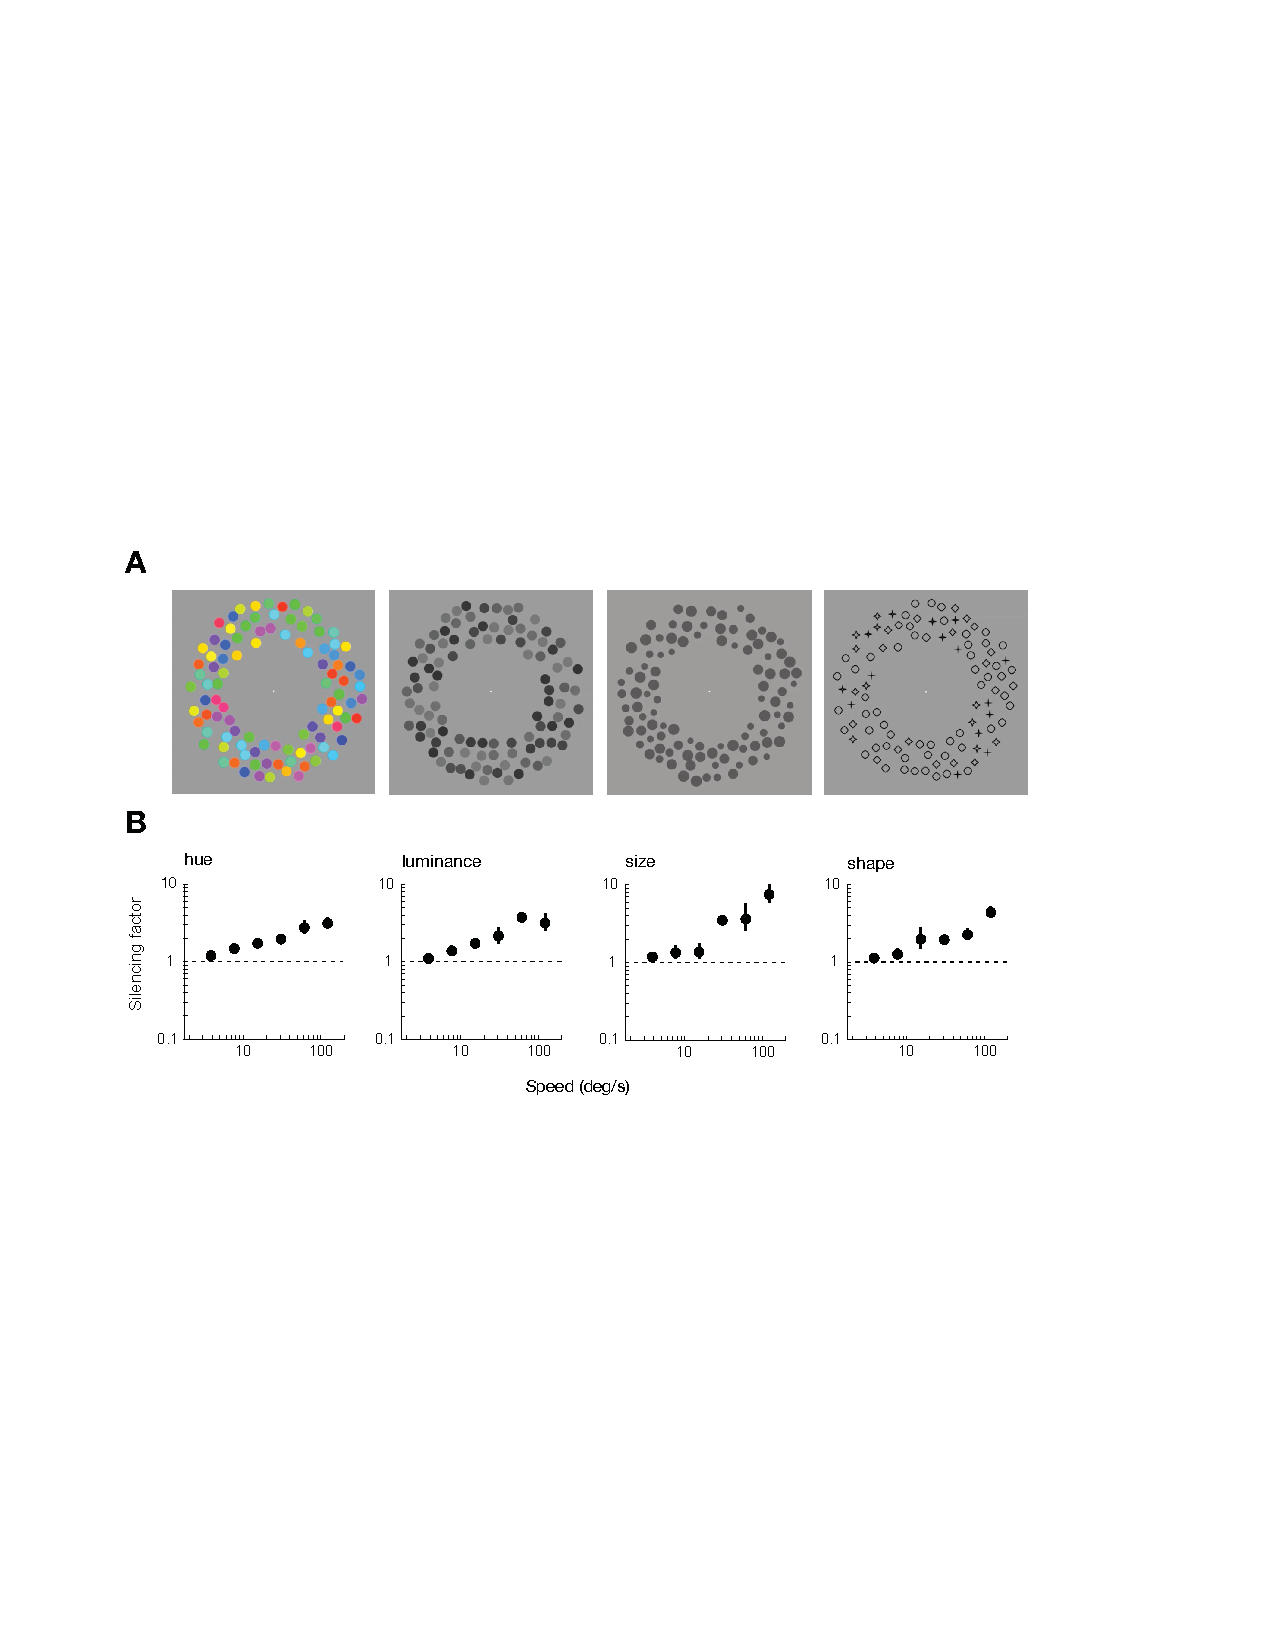
\includegraphics[width=\textwidth]{figures/fig1}
%\caption[Short figure name.]{This is a figure that floats inline and here is its caption.
%\label{fig:myInlineFigure}}
%\end{figure}


%% Requires fltpage2 package
%%
% \begin{FPfigure}
% 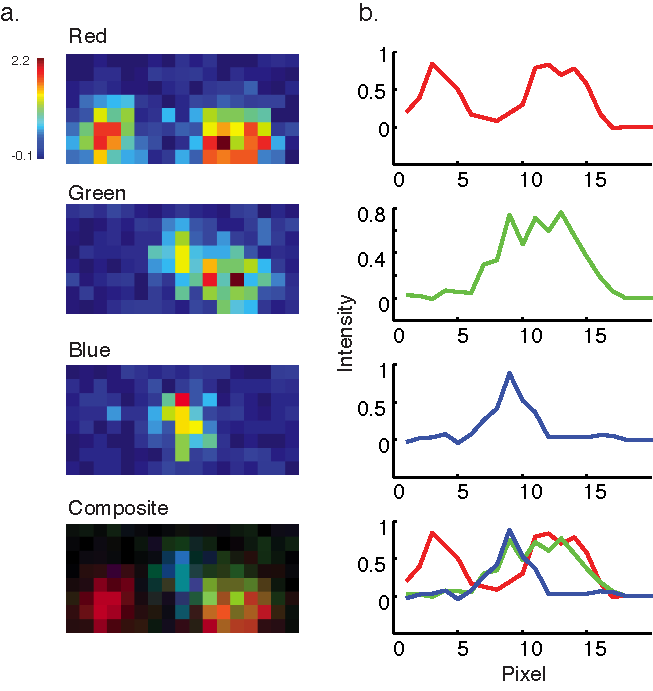
\includegraphics[width=\textwidth]{figures/figures/fullpage}
% \caption[Short figure name.]{This is a full page figure using the FPfigure command. It takes up the whole page and the caption appears on the preceding page. Its useful for large figures. Harvard's rules about full page figures are tricky, but you don't have to worry about it because we took care of it for you. For example, the full figure is supposed to have a title in the same style as the caption but without the actual caption. The caption is supposed to appear alone on the preceding page with no other text. You do't have to worry about any of that. We have modified the fltpage package to make it work. This is a lengthy caption and it clearly would not fit on the same page as the figure. Note that you should only use the FPfigure command in instances where the figure really is too large. If the figure is small enough to fit by the caption than it does not produce the desired effect. Good luck with your thesis. I have to keep writing this to make the caption really long. LaTex is a lot of fun. You will enjoy working with it. Good luck on your post doctoral life! I am looking forward to mine. \label{fig:myFullPageFigure}}
% \end{FPfigure}
% \afterpage{\clearpage}

\section{How do we generate hypotheses?}

In his preface to \emph{Astronomia Nova} (1609), Johannes Kepler described how he struggled to find an accurate mathematical description of planetary motion. Like most of his contemporaries, he started with the hypothesis that planets move in perfect circles. This necessitated extraordinary labor to reconcile the equations of motion with his other assumptions, ``because I had bound them to millstones (as it were) of circularity, under the spell of common opinion.'' It was not the case that Kepler simply favored circles over ellipses (which he ultimately accepted), since he considered several other alternatives prior to ellipses. Kepler's problem was that he failed to generate the right hypothesis.\footnote{In fact, Kepler had tried fitting an oval to his observations only to reject it, and then labored for another seven years before finally trying an ellipse and realizing that it was mathematically equivalent to an oval. As he recounted, ``The truth of nature, which I had rejected and chased away, returned by stealth through the back door, disguising itself to be accepted... Ah, what a foolish bird I have been!''} 

Kepler is not alone: the history of science is replete with examples of ``unconceived alternatives'' \citep{stanford10}, and many psychological biases can be traced to failures of hypothesis generation, as we discuss below. In this paper, we focus on hypothesis generation in the extensively studied domain of probabilistic inference. The generated hypothesis are a subset of a tremendously large space of possibilities. Our goal is to understand how humans generate that subset.

In general, probabilistic inference is comprised of two steps: hypothesis generation and hypothesis evaluation, with feedback between these two processes. Given a complete set of hypotheses $\mathcal{H}$ and observed data $d$, optimal evaluation is prescribed by Bayes' rule, which assigns a posterior probability $P(h|d)$ to each hypothesis $h \in \mathcal{H}$ proportional to its prior probability $P(h)$ and the likelihood of the observed data under $h$, $P(d|h)$:
\begin{align}
P(h|d) = \frac{P(d|h) P(h)}{\sum_{h' \in \mathcal{H}} P(d|h') P(h')}.
\end{align}
%start
%Therefore, an un-normalized probability $P(h|d) = P(d|h) P(h)$ for a specific hypothesis might be known or easy to find, but normalizing it to get a true probability estimate can be challenging as it requires  summing over all possible hypotheses. 
%end
Many studies have found that when $\mathcal{H}$ is supplied explicitly, humans can come close to the Bayesian ideal \citep[e.g.,][]{griffiths2006,griffiths2011,frank2012,petzschner2015,oaksford2007}.\footnote{This correspondence between human and Bayesian inference requires that the inference task must be one that is likely to have been optimized by evolution (e.g., predicting the duration of everyday events, categorizing and locating objects in images, making causal inferences), typically in domains where people have strong intuitive knowledge about the relative probabilities of hypotheses; asking humans to reason consciously about unnatural problems like randomness or rare events \citep[see][for discussion]{chater2006}, or carry out explicit updating calculations \citep{peterson1967man}, tends to produce deviations from the Bayesian ideal.} However, when humans must generate the set of hypotheses themselves, they cannot generate them all and instead generate only a subset, leading to judgment biases \citep{Thomas2008,Dougherty2003,carroll2015,koriat1980,weber1993,Gettys1979}. Some prominent biases of this kind are listed in Table~\ref{tab:biases}.
\begin{table}[htbp]
\centering
\caption{Biases in human hypothesis generation and evaluation.}
\label{tab:biases}
\begin{tabular}{p{.25\textwidth}>{\raggedright}p{.45\textwidth}>{\raggedright}p{.20\textwidth}}
\toprule
\textbf{Name}&\textbf{Description}& \textbf{Reference}\tabularnewline
\midrule \tabularnewline
Subadditivity& Perceived probability of a hypothesis is higher when the hypothesis is described as a disjunction of typical component hypotheses (unpacked to typical examples). & \citet{fox1998belief} \tabularnewline\tabularnewline
Superadditivity& Perceived probability of a hypothesis is lower when the hypothesis is described as a disjunction of atypical component hypotheses (unpacked to atypical examples). & \citet{super}, \citet{hadjichristidis1999opening} \tabularnewline\tabularnewline
Weak evidence effect& The probability of an outcome is judged to be lower when positive evidence for a weak cause is presented & \citet{weak}\tabularnewline\tabularnewline
Dud alternative effect & The judged probability of a focal outcome is higher when implausible alternatives are presented & \citet{dud}\tabularnewline\tabularnewline
Self-generation effect & The probability judgment over hypotheses that participants have generated themselves is lower as compared to the same hypotheses generated by others& \citet{koriat1980,conf} \tabularnewline\tabularnewline
Crowd within & The mean squared error of an estimate with respect to the true value reduces with the number of guesses. This reduction is more pronounced when the guesses are averaged across participants rather than within participants. & \citet{vul08}
\tabularnewline\tabularnewline
Anchoring and Adjustment & Generated hypotheses are biased by the hypothesis that is prompted at the start. & \citet{tversky} \tabularnewline
\bottomrule
\end{tabular}
\end{table}

Most previously proposed models of hypothesis generation rely on cued recall from memory based on similarity to previously observed scenarios \citep[c.f.][]{Thomas2008, gennaioli2010comes}. The probability of a generated hypothesis depends on the strength of its memory, and the number of such hypotheses generated is constrained by the available working memory resources. However, in most naturally encountered combinatorial hypothesis spaces, the number of possible hypotheses is vast and only ever sparsely observed. \cite{Goodman2008} showed that, when inferring Boolean concepts, people can generate previously unseen hypotheses by using compositional rules, instead of likening the situation to previously observed situations. So it seems that humans do not generate hypotheses only from the manageably small subset of previously observed hypotheses in memory and instead are able to generate hypotheses from the formidably large combinatorial space of all the conceivable possibilities. Given how large this space is, resource constraints at the time of inference suggest that only a subset are actually generated.

In this paper, we develop a normative theoretical framework for hypothesis generation in the domain of probabilistic inference, given fixed data, arguing that the brain copes with the intractability of inference by stochastically sampling hypotheses from the combinatorial space of possibilities \citep[see also][]{sanborn16}. Although this sampling process is asymptotically exact, time pressure and cognitive resource constraints limit the number of samples that can be generated, giving rise to systematic biases. Such biases are ``computationally rational'' in the sense that they result from a trade-off between the costs and benefits of computation---i.e., they are an emergent property of the expected utility calculus when costs of computation are taken into account \citep{Gershman2015,Vul2014,lieder2017anchoring}.
%%start2%%%%%%%%%%%%%%
We propose that the framing of a query leads to sampling specific hypotheses first, which biases the rest of the hypothesis generation process through correlations in the sampling process.
We discuss the properties of various sampler designs to explore the space of possible algorithms, and choose a specific design that can reproduce all the phenomena listed in Table~\ref{tab:biases}. We then test our theory's novel predictions in four experiments.
%%end2%%%%%%%%%%%%%%%%

\section{A rational process model of hypothesis generation}

Much of the recent work on probabilistic inference in human cognition has been deliberately agnostic about its underlying mechanisms, in order to make claims specifically about the subjective probability models people use in different domains \citep{chater2006}. Because the posterior distribution $P(h|d)$ is completely determined by the joint distribution $P(h,d) = P(d|h)P(h)$, an idealized reasoner's inferences can be perfectly predicted given this joint distribution. By comparing different assumptions about the joint distribution (e.g., the choice of prior or likelihood) under these idealized conditions, researchers have attempted to adjudicate between different models. Importantly, any algorithm that computes the exact posterior will yield identical predictions, which is what licenses agnosticism about mechanism. This method of abstraction is the essence of the ``computational level of analysis'' \citep{marr1976understanding}, and is closely related to the competence/performance distinction in linguistics and ``as-if'' explanations of choice behavior in economics.

The phenomena listed in Table~\ref{tab:biases} do not yield easily to a purely computational-level analysis, since different choices for the probabilistic model do not account for the systematic errors in approximating them. For this reason, we turn to ``rational process'' models \citep[see][for a review]{Griffiths2012BridgingCognition}, which make explicit claims about the mechanistic implementation of inference. Rational process models are designed to be approximations of the idealized reasoner, but make distinctive predictions under resource constraints. In particular, we explore how sample-based approximations lead to particular cognitive biases in a large space of hypotheses, when the number of samples is limited.
With an infinite number of samples, different sampling algorithms are indistinguishable as they all converge to the ideal response, but these algorithms display different behaviors at small sample sizes. We narrow the space of candidate sampling algorithms by studying these behaviors and comparing their predictions to observed cognitive biases.

\subsection{Monte Carlo methods}

We discuss Monte Carlo methods is detail in Chapter \ref{chap:approx}. Here we reiterate the basics. In their simplest form, sample-based approximations \citep[also known as \emph{Monte Carlo} approximations;][]{robert13}, take the following form:
\begin{align}
P(h|d) \approx \hat{P}_N(h|d) = \frac{1}{N}\sum_{n=1}^N \mathbb{I}[h_n=h],
\end{align}
where $\mathbb{I}[\cdot]=1$ when its argument is true (0 otherwise) and $h_n$ is a random hypothesis drawn from some distribution $Q_n(h)$.\footnote{This approach is straightforwardly generalized to sets of hypotheses: $\hat{P}_N(h \in H|d) = \frac{1}{N}\sum_{n=1}^N \mathbb{I}[h_n \in H]$, where $H \subset \mathcal{H}$.} When $Q_n(h) = P(h|d)$, this approximation is unbiased, meaning $\mathbb{E}[\hat{P}_N(h|d)] = P(h|d)$, and asymptotically exact, meaning $\lim_{N\rightarrow \infty} \hat{P}_N(h|d) = P(h|d)$.

In general, a bounded reasoner cannot directly sample from the posterior, because the normalizing constant $P(d) = \sum_{h} P(h,d)$ requires the evaluation of the joint probabilities of each and every hypothesis and is intractable when the hypothesis space is large. In fact, sampling from the exact posterior entails solving exactly the problem which we wish to approximate. Nonetheless, it is still possible to construct an asymptotically exact approximation by sampling from a Markov chain whose stationary distribution is the posterior; this method is known as \emph{Markov chain Monte Carlo} (MCMC). Before presenting a concrete version of this method, we highlight several properties that make it suitable as a process model of hypothesis generation. Some of these properties are shared with other sampling mechanisms, and others make MCMC more uniquely amenable.

%%start2%%%%%%%%%%%%%%
First, all Monte Carlo approximations including MCMC, are stochastic in the finite sample regime, producing ``posterior probability matching'' \citep{wozny2010,Denison2013,Moreno11,Vul2014}: hypotheses are generated with frequencies proportional to their posterior probabilities. Second, MCMC does not require knowledge of normalized probabilities at any stage and relies solely on an ability to compare the relative probabilities of two hypotheses. This is consistent with evidence that humans represent probabilities on a relative scale \citep{stewart06}. While this property is not true of all samplers, it is shared with a large class of sampling mechanisms based on importance sampling. Third, MCMC allows for feedback between the generation and evaluation processes. The evaluated probability of already-generated hypotheses influences if and how many new hypotheses will be generated, consistent with experimental observations \citep{hamrick2015think}. Here the properties of MCMC diverge more significantly from parallel sampling methods like importance sampling, where hypotheses are generated independently. Fourth, Markov chains (unlike parallel sampling mechanisms such as importance sampling) generate autocorrelated samples. This is consistent with autocorrelation in hypothesis generation \citep{multistability,vul08,Bonawitz2014}. Correlation between consecutive hypotheses that manifest as anchoring effects \citep[where judgments are biased by the initial hypothesis;][]{tversky} are replicated by MCMC approximations that are transiently biased (during the``burn-in'' period) by their initial hypothesis \citep{lieder2017anchoring,lieder2017empirical}. This seems to hold also true for the way in which participants update their internal models in causal learning tasks \citep{bramley2017formalizing}. Finally, work in theoretical neuroscience has shown how MCMC algorithms could be realized in cortical circuits \citep{buesing11,pecevski11,Moreno11}.

We will show how some of the biases in Table \ref{tab:biases} can be replicated with samplers that have some  subsets of these properties. Importantly, we will also show how a particular MCMC sampler can capture all of the biases in Table \ref{tab:biases}.

%%end2%%%%%%%%%%%%%%

%% Include here?  It doesn't require knowledge of normalized probabilities at any stage and relies solely on an ability to compare the relative probabilities of two hypotheses. This is reassuring because it is much more natural to expect that humans can gauge the relative probabilities of hypotheses better than their absolute probabilities \citep{stewart06}.

\subsubsection{Computational rationality of sampling}

We have emphasized properties that emerge in the finite sample regime because people tend to only generate a small number of hypotheses \citep{klein1999,ross96,Gettys1979,weber1993,dougherty1997}. Although this may seem to be manifestly sub-optimal, it can be justified within a ``computational rationality'' or ``resource-rational'' framework \citep{Vul2014,griffiths2015,Gershman2015,schulz2016simple}. If generating hypotheses is costly (in terms of time and cognitive resources), then the rational strategy is to generate the minimum number of samples necessary to achieve a desired level of accuracy. This implies that incentives or uncertainty should have systematic effects on hypothesis generation. For example, \citet{hamrick2015think} showed that people generated more hypotheses when they were more uncertain. By the same token, cognitive load \citep{sprenger2011} or response time pressure \citep{Dougherty2003} act as disincentives, reducing the number of generated hypotheses.

Despite our focus on the finite sample regime, it is also important to consider the asymptotic regime in order to explain the cases where human inference comes close to the Bayesian ideal. Monte Carlo algorithms are typically asymptotically exact; thus, they can accommodate unbiased inference when adequate cognitive resources are available. We do not claim, however, that all biases in human inference arise from adaptive allocation of cognitive resources. It seems likely that evolution has endowed the mind with some hardwired heuristics in order to avoid the cost of adaptive resource allocation \citep{gigerenzer09}.

\subsubsection{Comparison with particle filtering}

%%start2%%%%%%%%%%%%%%
A key feature of MCMC is that it produces hypotheses sequentially. As mentioned above, this gives it properties that distinguish it from parallel sampling mechanisms like importance sampling---specifically, the feedback between the generation and evaluation processes, and the autocorrelation of samples. It is therefore useful to 
%%end2%%%%%%%%%%%%%%
compare MCMC with \emph{particle filtering}, another Monte Carlo algorithm that generates hypotheses sequentially, and which has also been fruitfully applied to a number of domains in psychology, such as multiple object tracking \citep{vul2009explaining}, categorization \citep{sanborn2010rational}, and change detection \citep{brown09}. In order to clarify the distinction between the sequential nature of particle filtering and MCMC, we note that the sequential structure of particle filtering is dictated by the sequential nature of the generative process. For example, in multiple object tracking, the object positions are dynamic latent variables; particle filtering generates new hypotheses about the positions after each new data point is observed. Particle filters can also be used for inferring static parameters \citep{chopin2002sequential}, updating the Monte Carlo approximation as new data arrive. Note that in this case the generative process is still inherently sequential. In contrast, MCMC always involves sequential hypothesis generation, regardless of the structure of the generative process.

MCMC can also be used in conjunction with particle filters: the samples generated by the particle filter can be ``rejuvenated'' by applying a Markov chain operator that preserves the target distribution \citep{Abbott2011ExploringLearning,thaker2017online}. This process prevents degeneracy (collapse of the Monte Carlo approximation onto a few samples), a common problem in particle filtering. Here, the sequential nature of the Markov chain is relevant only locally to each step of the particle filter, orthogonal to the sequential nature with which the particle filter processes new data. In this paper, we focus on non-sequential generative models, with no online updating of data, in order to retain clarity on this point.
%end%%%%

\subsection{A specific Markov chain Monte Carlo algorithm}

The space of MCMC algorithms is vast \citep{robert13}, but for the purposes of modeling psychological phenomena many of the algorithms generate indistinguishable predictions. Our goal in this section is to specify one such algorithm, without making a strong claim that people adhere to it in every detail. We focus on qualitative features of the algorithm that align with aspects of human cognition. Nonetheless, we shall see that the algorithm makes accurate quantitative predictions about human probabilistic judgments.

The most well-known and widely-used version of MCMC is the Metropolis-Hastings algorithm. Here, at step $n$ in the Markov chain, new suggestions $h'$ are drawn from a proposal distribution $Q(h'|h_n)$, where $h_n$ is the hypothesis at step $n$. This proposal is accepted or rejected according to:
\begin{align}
P(h_{n+1}=h'|h_n) = \min\left[1, \frac{P(d|h')P(h') Q(h_n|h')}{P(d|h_n) P(h_n) Q(h'|h_n)} \right].
\end{align}

If the proposal is rejected, then the chain stays at the same hypothesis, $h_{n+1}=h_n$. Although the posterior cannot be directly evaluated, we assume it is known up to a normalizing constant, since $P(h|d) \propto P(d|h) P(h)$. The acceptance function forces moves to higher probability hypotheses, while also stochastically exploring lower probability hypotheses. This process repeats until $N$ samples have been generated. 
%%start
In the limit of large $N$, the amount of time the chain spends at a particular hypothesis is proportional to its posterior probability. If $N$ is not large enough, then the samples are affected by the initialization, leading to biased estimates of the posterior probability.
%end%%
The unique members of the set of accepted samples constitute the generated hypotheses, and the number of times they appear provides their judged probability.

%%start%%%%%%%%%%%%%%
We recap here two psychologically appealing properties of the algorithm mentioned in the previous section. First, we see that it relies solely on being able to gauge relative probabilities and not on having good estimates for any absolute probabilities. Second, the acceptance function engenders an interaction between generation and evaluation by ensuring that if one is at a high probability hypothesis, proposals are more likely to be rejected and therefore not generated%%start
\footnote{A low acceptance rate only implies that proposals are lower probability than the current state of the Markov chain, not that the current hypothesis necessarily has a high probability globally. There may always be higher probability hypotheses that the proposal distribution fails to propose. Conversely, a high acceptance rate does not necessarily imply a poor current hypothesis. For example, if the proposal distribution is proportional to the posterior distribution, then all proposals will be accepted.}
%%end
% .This follows the intuition that, if one finds a good (high probability) hypothesis, one is less likely to generate more hypotheses. Conversely, if one is at a bad (low probability hypothesis), more proposals will be accepted. Third, we see that the chain will be trivially autocorrelated as long as the rejection rate is non-zero. That is, the same hypothesis will appear consecutively in the chain, giving it some autocorrelation. A more sophisticated autocorrelation can also be induced by preferentially proposing hypotheses (from the proposal distribution) that are correlated with the current hypothesis.

%The hypotheses generated and the probabilities returned at a specific chain length $N$ are obtained by averaging over the results of multiple ($M$ in number) chains, each being run for $N$ steps. 
%In the case of unpacked hypotheses, each of the example hypotheses (total $K$ unpacked examples) initializes a new chain. Each of the $K$ chains is simulated $M$ times, initialized at the same example hypothesis and run for $\lfloor N/K \rfloor $ steps (with the remainder added randomly to one of the $K$ chains so that over the $M$ simulations, each chain runs for $N/K$ steps in expectation). We do not account for order effects - i.e. the order in which the examples are presented does not affect the model's predictions. To balance this assumption, we randomize the order of the presented examples in our experiments to nullify any order effect that may empirically be present. To minimize confounding effects, the packed control is modeled as similarly as possible - with only the initialization being different in each . Again, we have $K$ chains, each of which is run $M$ times, but each chain is initialized by randomly sampling the initialization distribution (which in our case is the prior over the focal space) instead of with one of the prompted examples, and similarly run for $\lfloor N/K \rfloor $ steps (with the remainder added randomly to one of the $K$ chains so that over the $M$ simulations, each chain runs for $N/K$ steps in expectation) each.

The next step is to specify the proposal distribution. For simplicity, we assume that the proposal is symmetric, $Q(h'|h) = Q(h|h')$. This reduces the acceptance function to:
\begin{equation}
\label{eq:acceptance}
P(h_{n+1}=h'|h_n) = \min\left[1, \frac{P(d|h')P(h')}{P(d|h_n) P(h_n)} \right].
\end{equation}

We also assume that the proposal distribution is ``local'': the proposal distribution preferentially proposes hypotheses that are in some way ``close'' to the current one. This ensures that the hypothesis generated next is close to the current one with high probability. The alternative possibility is to instead have a ``global'' proposal distribution - for example one that proposes the next hypothesis uniformly at random from the space of all possible hypotheses, instead of favoring those closer to the current one.

MCMC algorithms always exhibit some autocorrelation 
%%start%%%
as long as the acceptance ratio is less than one (irrespective of the details of the proposal distribution), because the same state occurs consecutively when a proposal is rejected.
%%end%%
However, we are also interested in the next \textit{new} hypothesis that is generated, not exact repetitions of the same hypothesis. A more nuanced notion of autocorrelation takes into account the fact that sampled hypotheses can be ``similar'' (though not identical) when the proposal distribution is centered on a local neighborhood of the current hypothesis, as opposed to if the proposal is a ``global'' one. This kind of locality in determining the next state given the current one, has been studied previously in the context of traversing and searching semantic networks \citep{abbott2015random} and combinatorial spaces \citep{smith2013multiply}. This locality has been shown to be optimal as a foraging strategy \citep{hills2012optimal} as well as consistent with human behavioral data. Since the generation of hypotheses is largely analogous to a search through the combinatorial space of conceivable possibilities, locality in the proposal distribution that moderates this search can be expected.

The question then is how we should define locality. This is relatively easy to answer in domains where the inference is over a one-dimensional continuous latent variable like in \cite{Lieder2013}; for example, one can use a normal distribution centered at the current hypothesis. For the discrete combinatorial hypothesis spaces studied in this paper, we assume that there is some natural clustering of the hypotheses based on the observations they tend to generate (their centroids). We use the Euclidean distance between centroids as a measure of distance between clusters. In our simulations, we assume for simplicity that all hypotheses within a cluster are equidistant and that all clusters are equidistant from each other. The proposal distribution chooses hypotheses in the same cluster with a higher probability than those outside the cluster, but it treats all hypotheses within a cluster equiprobably. While this structure induces locality in the proposal distribution, we are not making a strong claim about the nature or role of clustering in hypothesis generation. We speculate about more sophisticated proposal distributions in the section on limitations and future extensions. 

%Through the course of our simulations, we subjectively compare the results from our model to a Markov chain that uses such a ``global'' proposal in order to highlight the importance of having correlation between consecutively generated hypotheses in explaining the effects noted in Table \ref{tab:biases}.

Finally, we need to specify how the chain is initialized. For cases where a hypothesis is presented explicitly or primed in the query, we assume that the chain starts at that hypotheses.
%%start%%%%%%%
If there are several hypotheses (say $n$ in number) that have been presented explicitly in the query, we assume
% that they are all treated equivalently (neglecting order effects in our first approximation) and
that a different chain starts from each of these hypotheses and runs for $\frac{N}{n}$ steps each, giving a total of $N$ samples. However, in cases where no hypotheses are explicitly prompted, we assume that the initial hypothesis is drawn from the prior over the hypotheses instead of initializing at a prompted example. This assumption is consistent with evidence that hypotheses with high base rates are more likely to be generated \citep{weber1993}. In order to maximize similarity to the corresponding ``explicitly prompted'' version of the question and keep the number of new initializations the same, $n$ such chains are run for $\frac{N}{n}$ steps to give a total of $N$ samples.
%end%%%%%%%%%%%
There may also be initialization schemes that mix explicit prompts and sampling from the prior---for example a prompt that encourages sampling from a specific subset of the hypothesis space. We speculate about more sophisticated initialization schemes in the section on limitations and future extensions.

%Eric2: Should we say something about anchoring and adjustment here already, given Reviewer 2's comments?

\section{Model simulations of historically observed effects}

In this section we apply our model to a range of empirical phenomena, using a disease-symptom Bayesian network as our running example. For each simulation, we run the Markov chain many times and average the results, in order to emulate multiple participants in an experiment.

\subsection{Diagnostic hypotheses in a disease-symptom network}

Our model is generally applicable to domains where the inference is carried out over a large space of possibilities that is sparsely observed and thus requires one to generate previously unobserved possibilities. A data set containing medical symptoms is a prototypical example of this problem: a patient could have any combination of more than one disease and many such combinations will not have been encountered before by an individual clinician. This combinatorial structure makes medical diagnosis computationally difficult---exact inference in a Bayesian network is known to be NP-hard \citep{cooper1990complexity}. To address this problem, approximate probabilistic inference algorithms (including Monte Carlo methods) are now widely-established \citep[e.g.,][]{Shwe1991, Jaakkola1999, Heckerman1990}. It is therefore reasonable to conjecture that diagnostic reasoning by humans could be captured by similar approximate inference algorithms. Suggestively, a number of the judgment biases listed in Table \ref{tab:biases} have been documented in clinical settings \citep{redelmeier1995probability,elstein1978medical,weber1993}; our goal is to investigate whether the MCMC model can reproduce these biases.

In the disease-symptom network, the observations are the presence or absence of symptoms and the latent variables are the presence or absence of diseases ($S$ possible symptoms and $D$ possible diseases). The diagnostic problem is to compute the posterior distribution over $2^D$ binary vectors, where each vector encodes the presence ($h_d=1$) or absence ($h_d=0$) of diseases $d = 1,\ldots,D$. The diseases are connected to the symptoms via a noisy-or likelihood, following \cite{shwe1991probabilistic}:
\begin{align}
P(k_s = 1|h) = 1 - (1-\epsilon) \prod_{d=1}^D (1-w_{ds})^{h_d},
\end{align}
where $k_s = 1$ when symptom $s = 1, \ldots, S$ is present (0 otherwise), $\epsilon \in [0,1]$ is a base probability of observing a symptom, and $w_{ds} \in [0,1]$ is a parameter expressing the probability of observing symptom $s$ when only disease $d$ is present. Intuitively, the noisy-or likelihood captures the idea that each disease has an independent chance to produce a symptom.

As our goal is to use this set-up purely for illustrative purposes, we use a simplified fictitious disease-symptom data set designed to resemble real-world contingencies (Table~\ref{tab:qmr}). We designated two distinct clusters of four diseases each (gastrointestinal diseases and respiratory diseases); these two clusters have largely disjoint sets of symptoms, and the symptoms within a cluster are largely overlapping. We allow any combination of diseases to be present, making even this small number of diseases a fairly large space of 256 possible hypotheses.

\begin{table}[htbp]
%\setstretch{\ddoublespacing}
\caption{Parameters used for noisy-or model.}
  \begin{center}
\begin{tabular}{>{\raggedright}m{0.16\textwidth} m{0.07\textwidth} m{0.04\textwidth} m{0.05\textwidth} m{0.04\textwidth} m{0.08\textwidth} m{0.08\textwidth} m{0.08\textwidth} m{0.1\textwidth} m{0.04\textwidth}} 
  \toprule

     \multirow{2}{*}{Symptoms} &
      \multicolumn{9}{c}{Diseases} \\
 & lung cancer & TB & resp. flu & cold & gastro-enteritis & stomach cancer & stomach flu & food poisoning & base \\
\midrule
Prior & 0.001 & 0.05 & 0.1 & 0.2 & 0.1 & 0.05 & 0.15 & 0.2 & 1.0\\
%\hline \hline
cough & 0.3 & 0.7 & 0.05 & 0.5 & 0.0 & 0.0 & 0.0 & 0.0 & 0.01 \\
%\hline
fever & 0.0 & 0.1 & 0.5 & 0.3 & 0.0 & 0.0 & 0.1 & 0.2 & 0.01 \\
%\hline
chest pain & 0.5 & 0.5 & 0.0 & 0.0 & 0.0 & 0.0 & 0.0 & 0.0 & 0.01 \\
%\hline
short breath & 0.5 & 0.2 & 0.0 & 0.0 & 0.0 & 0.0 & 0.0 & 0.0 & 0.01 \\
%\hline
nausea & 0.0 & 0.0 & 0.2 & 0.1 & 0.5 & 0.1 & 0.5 & 0.7 & 0.01 \\ 
%\hline
fatigue & 0.0 & 0.0 & 0.2 & 0.3 & 0.1 & 0.05 & 0.2 & 0.4 & 0.01 \\
%\hline
bloating & 0.0 & 0.0 & 0.0 & 0.0 & 0.3 & 0.05 & 0.1 & 0.5 & 0.01 \\
%\hline
abdom. pain & 0.0 & 0.0 & 0.01 & 0.0 & 0.1 & 0.5 & 0.0 & 0.0 & 0.01 \\
%\hline
\bottomrule
\end{tabular}
\end{center}
\label{tab:qmr}

\end{table}

\subsection{Subadditivity}

As described above, a resource-rational algorithm will arrest computation after a small number of samples, once accuracy is balanced against the cost of sampling \citep{Vul2014}. This gives rise to \emph{subadditivity} (see Table \ref{tab:biases}): the probability of a disjunction (in ``packed'' form) is judged to be less than the probability of the same disjunction presented explicitly as the union of its sub-hypotheses (in ``unpacked'' form) \citep{tversky94,Dougherty2003}, despite the fact that mathematically these are equal. For example, the probability of a gastrointestinal disease is judged to be less than the sum of the probabilities of each possible gastrointestinal disease.

Let us define a few terms here that we use in our simulations of these unpacking effects. The space of hypotheses that the disjunction refers to is called the \textit{focal space} of the query. For example, when queried about the probability of a gastrointestinal diseases, the focal space is the set of all hypotheses that include at least one gastrointestinal disease. When unpacking this disjunction, we do not unpack to every single member of the focal space. Instead, we unpack to a few examples and to a \emph{catch-all hypothesis} that refers to all other members of the focal space that were not explicitly unpacked. 
%start%%
For example: ``Food poisoning, stomach cancer or any other gastrointestinal disease'' where a few example components of the focal space are unpacked and explicitly prompted in the question (food poisoning and stomach cancer) and presented along with a catch-all hypothesis (any other gastrointestinal disease).\footnote{In this paper, we study what is termed ``implicit'' subadditivity, where the unpacked query is framed as a conjunction of mutually exclusive sub-hypotheses, in contrast to ``explicit'' subadditivity, where each mutually exclusive sub-hypothesis is queried separately and the numerical estimates from each query are then added together. Explicit subadditivity could be modeled the same way as implicit subadditivity if we assume that the number of samples generated over the separately queried sub-hypotheses is equal to the net number of hypotheses generated in response to the conjunction, and that no samples are carried over in between the separately queried hypotheses.}
%%end%%%

Our model offers the following explanation of subadditivity: when a packed hypothesis is unpacked to typical examples and a catch-all hypothesis, the typical examples (that are part of the focal space) are explicitly prompted, causing the Markov chain to start there and thus include them in the cache of generated hypotheses.
%start%%%%%%%
If the examples are not explicitly prompted and instead a packed hypothesis is presented, the chain initializes with a random sample from the prior. The chain is thus likely to start from a fairly typical (high prior probability) hypothesis; however, with some probability it may fail to generate all the high probability hypotheses. Deterministically initializing the chain at a typical (high probability) hypothesis, ensures that the chain generates high probability hypotheses in the focal space and thus results in a larger probability judgment for that focal space.
%end%%%%%%%
This effect can also be replicated by a parallel sampling algorithm as seen in \cite{Thomas2008}. Here explicitly prompted hypotheses (under the unpacked condition) are appended to the other samples that would have been generated without prompting (under the packed condition), leading to more hypotheses in the focal space being generated in the unpacked condition and therefore raising the probability estimate under that condition.

To illustrate this effect in our medical diagnosis model, consider the following queries: 
\begin{itemize}
\item Packed query: Given the symptoms \emph{fever, nausea} and \emph{fatigue}, what is the probability that these symptoms were caused by the presence of a gastrointestinal disease? 
\item Unpacked query (typical examples): Given the symptoms \emph{fever, nausea} and \emph{fatigue}, what is the probability that these symptoms were caused by the presence of food poisoning, stomach flu, or any other gastrointestinal diseases?
\end{itemize}
The difference between the probability estimates between these two conditions is shown in Figure~\ref{fig:subadd}.

\begin{figure}
\centering
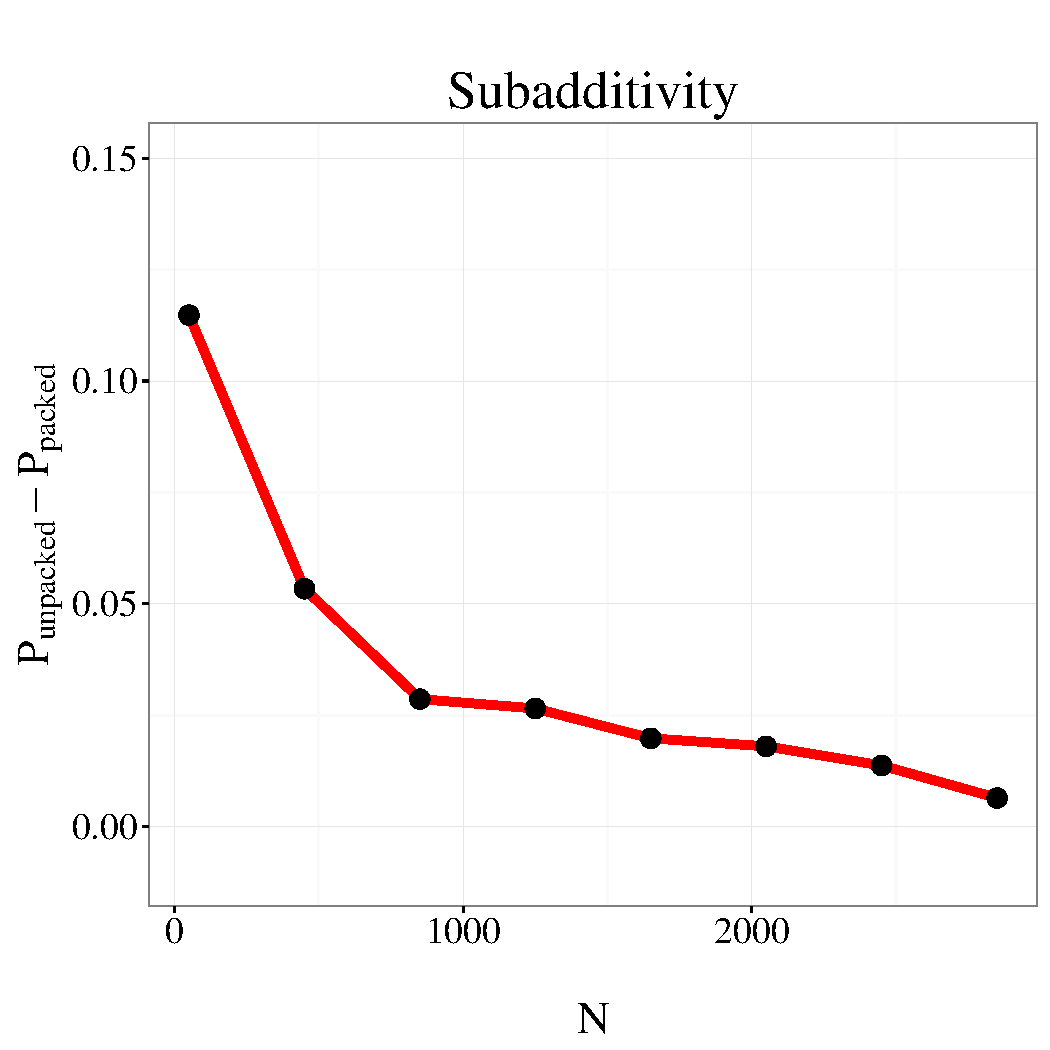
\includegraphics[scale = 0.5]{figures/sub.pdf}
\caption{\textbf{Subadditivity}. MCMC estimates were made for the following queries: Given the symptoms \emph{fever, nausea} and \emph{fatigue}, (a) Packed: what is the probability that these symptoms were caused by the presence of a gastrointestinal disease? (b) Unpacked to typical examples: what is the probability that these were caused by the presence of food poisoning, stomach flu, or any other gastrointestinal diseases? The estimate for the unpacked condition is higher than that of the packed condition. The difference between these estimates is represented by the red line. This effect diminishes as the number of samples increases.}
\label{fig:subadd}
\end{figure}

Experiments in \cite{Dougherty2003} show that the effect size of subadditivity decreases as the participants are given more time to answer the question. In our model, as more samples are taken, it becomes more and more likely that the packed chain also finds the high probability examples prompted in the unpacked scenario on its own. So the head-start given to the unpacked chain gets gradually washed out and the effect size of subadditivity decreases. If we assume that as more time passes, people take more samples (up until a resource-rational limit on the number of samples), and that the time-points measured are before the resource-rational sample limit is met, our model replicates these time-dependence effects as seen in Figure \ref{fig:subadd}.

\subsection{Superadditivity and related effects}

Taking a limited number of samples with an MCMC sampler can also give rise to an effect opposite to the one described in the previous section, known as \emph{superadditivity} (see Table \ref{tab:biases}): the probability of a disjunction (in ``packed'' form) is judged to be \textit{greater} than the probability of the same disjunction presented explicitly as the union of its sub-hypotheses (in ``unpacked'' form) \citep{super,hadjichristidis1999opening}, despite the fact that mathematically they should be equal. This effect occurs when unpacking to atypical (low probability) examples and subadditvity prevails when unpacking to typical (high probability) examples.

The key feature that produces this effect is the acceptance function of the MCMC sampler and the feedback it causes between the generation and evaluation processes. If a chain is at a low probability hypothesis (such as when a low probability hypothesis is explicitly prompted in the form of an atypical unpacking), the chain is likely to accept more of the proposals made by the proposal distribution. Therefore, this chain could generate many alternate hypotheses outside the focal space. In contrast, a chain at a higher probability hypothesis (for example, if it was randomly initialized in the focal space instead of being initialized at a particularly atypical example) will reject more of these proposals and remain at the initial hypothesis. So most of these proposals will not be generated. The probability estimate for the focal space $\mathcal{A}$ is given by 

\begin{align}
\sum_{h \in \mathcal{A}} \hat{P}(h | d) = 
\sum_{h \in \mathcal{A}}\frac{1}{N}\sum_{n=1}^N \mathbb{I}[h_n=h] = 
\frac{\sum_{h \in \mathcal{A}} \sum_{n=1}^N \mathbb{I}[h_n=h]}
{\sum_{h \in \mathcal{A}} \sum_{n=1}^N \mathbb{I}[h_n=h] + \sum_{h' \notin \mathcal{A}} \sum_{n=1}^N \mathbb{I}[h_n=h']}
\end{align}

Being in $\mathcal{A}$ or not divides the total hypothesis space of $\mathcal{H}$ into two mutually exclusive parts. Therefore, the generation of more hypotheses outside the focal space (on average) when initialized at a consistently low probability (atypical) hypothesis in the focal space lowers the resulting probability estimate of the focal hypothesis space. This results in superadditive judgments.
 
To elucidate this effect in our medical diagnosis model, we use the following ``unpacked to atypical examples'' query: Given the symptoms \emph{fever, nausea} and \emph{fatigue}, what is the probability that these symptoms were caused by the presence of gastroenteritis, stomach cancer, or any other gastrointestinal disease? The difference between the probability estimates from the two conditions is shown in Figure \ref{fig:superadd}.

\begin{figure}
\centering
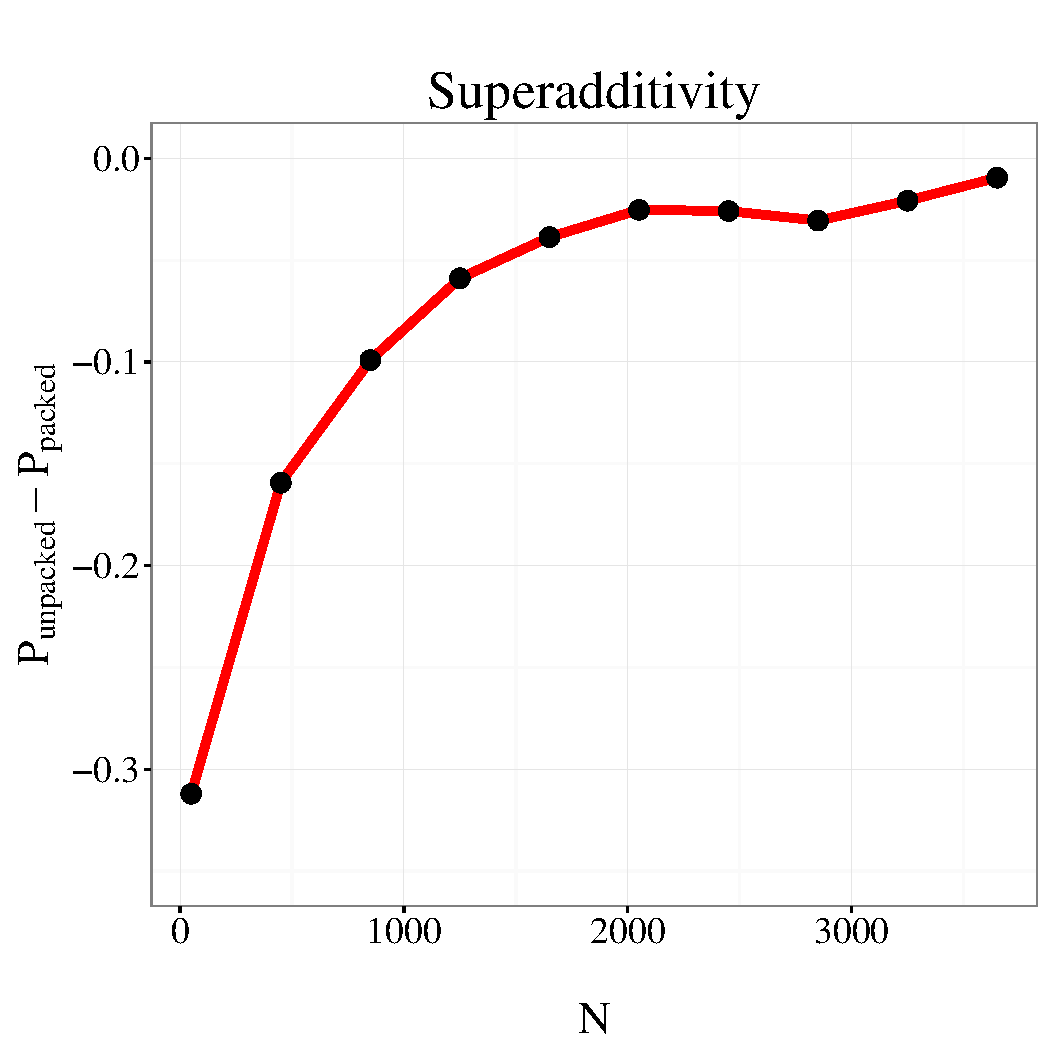
\includegraphics[scale = 0.5]{figures/super.pdf}
\caption{\textbf{Superadditivity}. MCMC-estimates were made for the following queries: Given the symptoms \emph{fever, nausea} and \emph{fatigue}, (a) Packed: What is the probability that these symptoms were caused by the presence of gastrointestinal disease? (b) Unpacked to atypical examples: What is the probability is that these symptoms were caused by the presence of gastroenteritis, stomach cancer, or any other gastrointestinal disease? The estimate for the unpacked condition is lower than that of the packed condition. The difference between these estimates is represented by the red line. This effect diminishes as the number of samples increases.}
\label{fig:superadd}
\end{figure}

Previous accounts of subadditivity \citep[e.g.,][]{Thomas2008, MINERVAsub} cannot explain superadditivity; any unpacked example only increases the probability judgment of the unpacked query with respect to the packed query. This weakness of MINERVA-DM has been observed by \cite{Costello2014} in the context of its failure to model binary complementarity---an effect which their noise-based analysis can capture. However, their analysis still fails to completely capture superadditivity, as it constrains unpacked judgments to be greater than (and, only for binary complements, equal to) the packed judgment, never less than the packed judgment. 
%start2
Our modeling of this effect hinges on the fact that MCMC allows for feedback between the generation and evaluation processes---the evaluated probability of already generated hypotheses influences how many new hypotheses will be generated. This property is not shared by  parallel sampling algorithms. However, other samplers (besides MCMC algorithms) that exhibit correlated sampling may exhibit similar behaviors \citep[see for example][]{Bonawitz2014}.
%end2
%ES2: I like that addition, maybe we could spell it out a little further.

\cite{super} explain superadditivity by suggesting that atypical examples divert attention from more typical examples and thus lower the probability estimate. But an explanation at the level of a rational process model is, to our knowledge, lacking in the literature. 


Some other cognitive effects can also be modeled by the same mechanism that gives rise to superadditivity. One example is the \emph{weak evidence effect}: the perceived probability of an outcome is lowered by the presence of evidence supporting a weak cause. %%start
 \cite{weak} explain this effect as follows: mentioning evidence in support of a specific weak cause drives people to focus disproportionately on it and thus they fail to think about other good candidates in the focal space of possible causes. Our model replicates this effect by initializing at the weak cause, or low-probability hypothesis, resulting in a lower probability judgment of the focal space by the same mechanism as in the superadditivity effect. However, the added evidence should normatively increase the probability of the cause it supports. Since the evidence is weak, this increase is small and the cause still remains low probability. Therefore, the superadditivity effect overwhelms this small increase in probability of the specific hypothesis and instead lowers the probability estimate of the focal space overall. This causes the final judged probability to be lower than if the positive evidence had not been presented and the chain was initialized randomly (on average at a higher probability hypothesis than the presented weak one) in the focal space.
 %%%end%%%%

To elucidate this effect in our medical diagnosis model, we use the following query:
\begin{itemize}
\item Control: Given the symptoms \emph{fever, nausea}  and \emph{fatigue}, what is the probability that these symptoms were caused by the presence of gastrointestinal disease?
\item Evidence for a weak cause: Given the symptoms \emph{fever, nausea}  and \emph{fatigue}, what is the probability that these symptoms were caused by the presence of gastrointestinal disease, assuming the patient's grandmother was diagnosed with stomach cancer?
\end{itemize}
The increase in support of the weak cause (stomach cancer), by making available the presence of familial history, is implemented in our model by increasing the prior probability of stomach cancer in this patient from 0.05 to 0.06 (see Table \ref{tab:qmr}). While this small change is not expected to elicit a large difference in the probability of gastrointestinal diseases between the two cases, it certainly does make it more (rather than less) probable compared to the control. However, it also causes the chain to be initialized at the weak hypothesis of stomach cancer by prompting it, resulting in the generation of more alternative hypotheses outside the focal space and a lower probability judgment than in the first case (Figure \ref{fig:weak}).

\begin{figure}
\centering
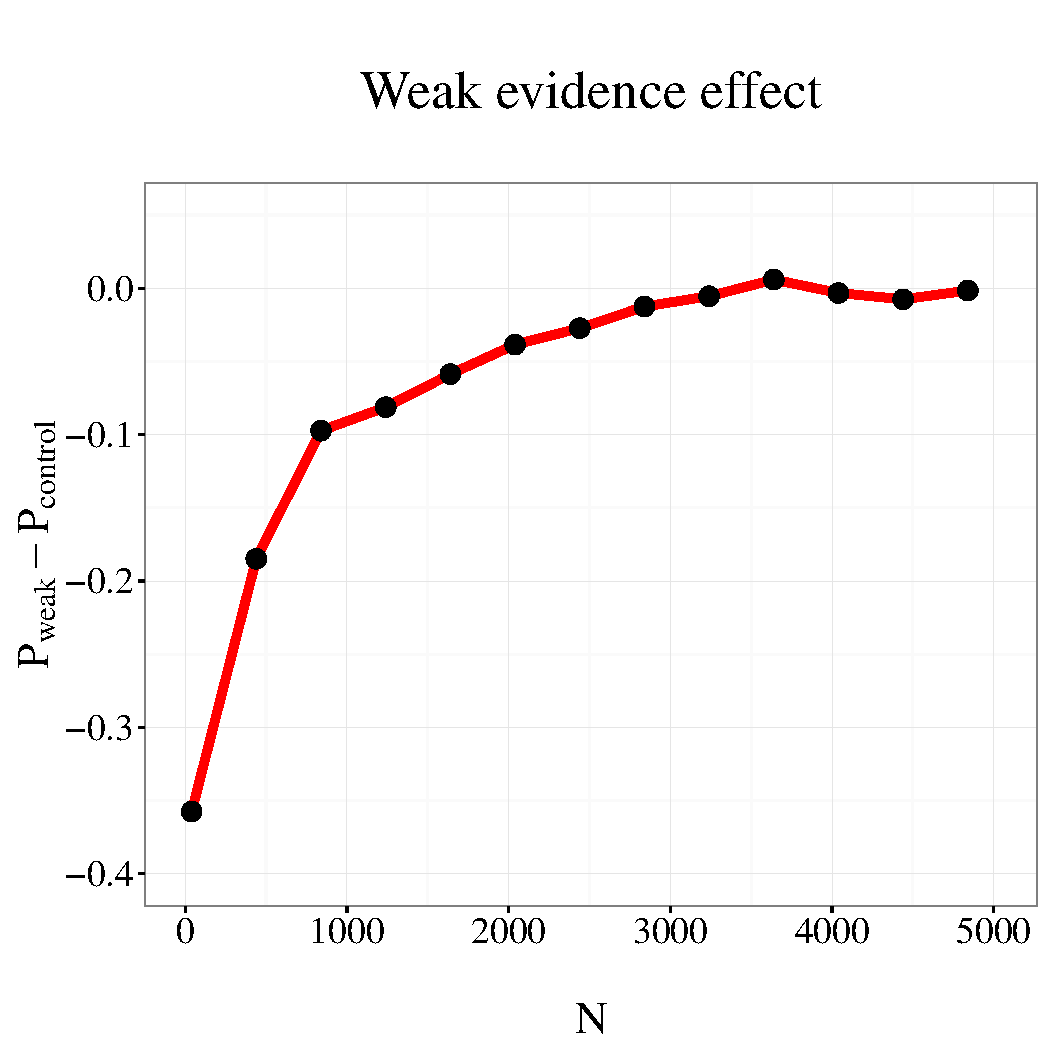
\includegraphics[scale = 0.5]{figures/weak.pdf}
 \caption{\textbf{Weak evidence effect}. MCMC estimates were made for the following queries: Given the symptoms \emph{fever, nausea}  and \emph{fatigue}, (a) Control: What is the probability that these symptoms were caused by the presence of gastrointestinal disease? (b) Evidence for a weak cause: What is the probability that these symptoms were caused by the presence of gastrointestinal disease, assuming the patient's grandmother was diagnosed with stomach cancer? The increase in support of the weak cause (stomach cancer) is modeled by increasing the prior probability of stomach cancer from 0.05 to 0.06. The estimate from the weak evidence chain is lower than that from the control chain. The difference between these estimates is represented by the red line. The effect diminishes as the number of samples increases.}
 \label{fig:weak}
\end{figure}

Another such bias is the \emph{Dud alternative effect}: presenting low probability (or ``dud'') alternate hypotheses increases the perceived probability of the focal space of hypotheses \citep{dud}. This can be viewed as the superadditivity effect in the complement (alternate) hypothesis space. The queries being contrasted here are initialized in the space complementary to the focal space---i.e., the space of alternatives. Initialization at a low probability alternative when it is explicitly prompted in the question results in a superadditive judgment (i.e., a lower probability judgment) of the complement space. This lower probability estimate for the complement space entails a higher probability estimate for the focal space.
%%start
The assumption here is that the same chain is used to gauge the probability of both binary complements, by grouping the generated hypotheses into being either inside or outside the focal space and calculating the net- probability of each group. The framing simply alters the initialization of the chain. This assumption ensures that probability judgments over complementary spaces add up to one, in accordance with behavioral experiments that demonstrate binary complementarity in human judgments \citep{tversky94}.
%%end%%%%%%%%%

To elucidate this effect in our medical diagnosis model, we use the following queries:
\begin{itemize}
\item Control: Given the symptoms \emph{fever, nausea} and \emph{fatigue}, what is the probability that the patient has a respiratory disease (as opposed to the symptoms being caused by the presence of a gastrointestinal disease)?
\item Dud alternative: Given the symptoms \emph{fever, nausea} and \emph{fatigue}, what is the probability that the patient has a respiratory disease (as opposed to the symptoms being caused by the presence of gastroenteritis, stomach cancer, or any other gastrointestinal disease)?
\end{itemize}
We see in Figure \ref{fig:dud} that the model predicts that the scenario with dud alternatives produces higher probability judgments than the control. Findings in \cite{dud} also suggest that the magnitude of this effect decreases with the amount of processing time given to participants. The model also replicates this phenomenon, if we assume that more time means more samples, and that the time points queried are before the resource-rational limit on the number of samples is reached.

\begin{figure}
\centering
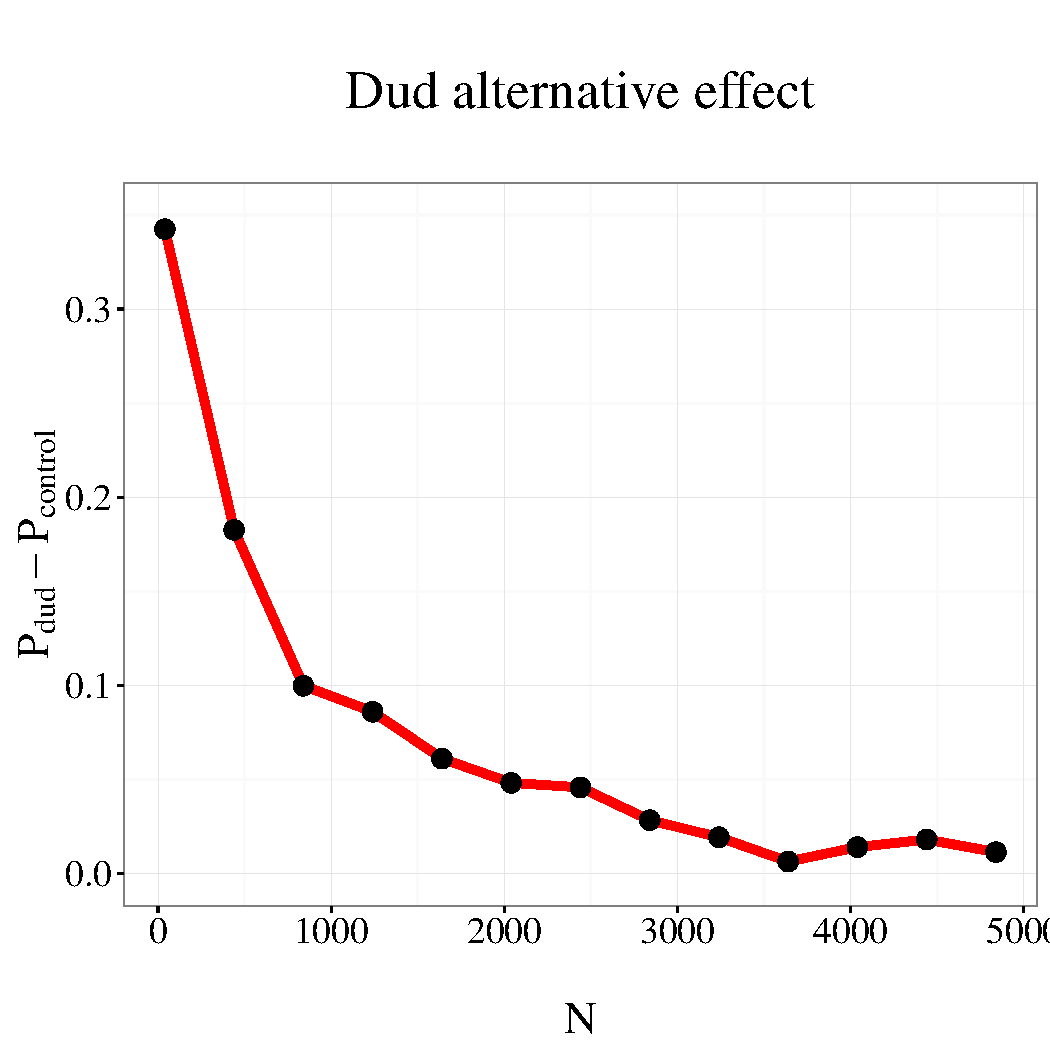
\includegraphics[scale = 0.5]{figures/dud.pdf}
\caption{\textbf{Dud alternative effect}. MCMC estimates were made for the following queries: Given the symptoms \emph{fever, nausea}  and \emph{fatigue}, (a) Control: What is the probability that the patient has a respiratory disease (as opposed to the symptoms being caused by the presence of a gastrointestinal disease)?,  (b) With dud alternatives: What is the probability that the patient has a respiratory disease (as opposed to the symptoms being caused by the presence of gastroenteritis, stomach cancer, or any other gastrointestinal disease)? The estimate from the control chain is higher than from the chain for which dud alternatives are presented. The difference between these estimates is represented by the red line and the effect diminishes as the number of samples increases}
\label{fig:dud}
\end{figure}

Our model currently only captures cases of binary complementarity where it's obvious to participants that complementarity holds. If this complementarity is obvious, then they can use the same chain, and if the complementarity isn't obvious, then they use a new chain. If this new chain is not suggestively unpacked, approximate binary complementarity should still hold. It is an interesting challenge to understand when humans might re-use the same chain and when they might use a new chain, and when they might use some intermediate between the two. This is part of our ongoing research.

\subsection{Self-generation of hypotheses}

In this section, we focus on the \emph{self-generation effect}: the probability judgment of a set of hypothesis that are generated and reported by a subject themselves is lower than when the same set of reported hypotheses is presented to a new subject \citep{conf,koriat1980}. Our model provides the following explanation: Self-reported hypotheses generated by a chain are the modes it discovers after having explored the space and having generated several alternate hypotheses. However, in a situation where these high probability hypotheses are directly presented, the chain starts at the mode and is likely to get stuck---i.e., not accept any of the proposals and thus not generate them at all. This, in the small sample limit, results in the generation of fewer alternate hypotheses. As in the previous section, fewer alternate hypotheses lead to a higher probability judgment.

\begin{figure}
\centering
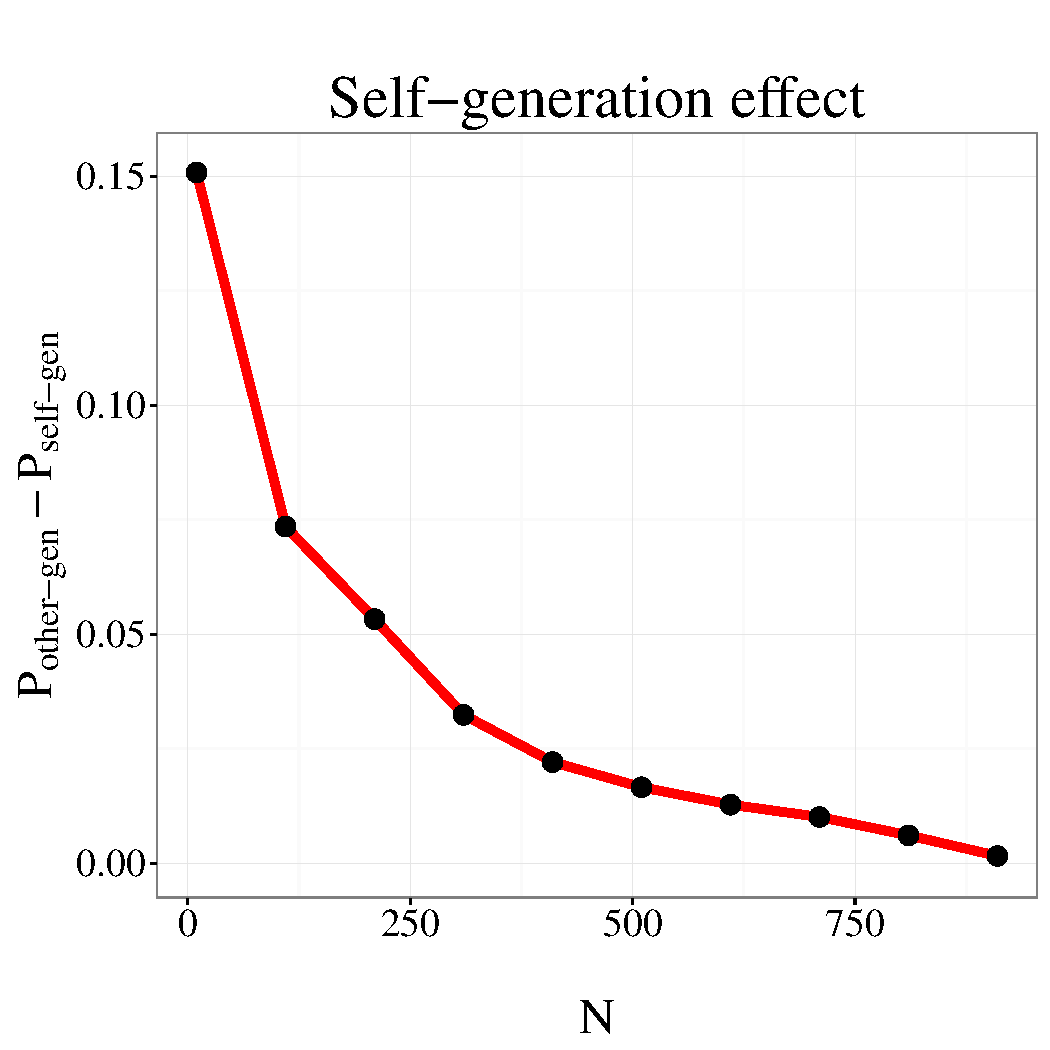
\includegraphics[scale = 0.5]{figures/confidence.pdf}
\caption{\textbf{Self-generation effect}. MCMC estimates for the following query: Given the symptoms \emph{fever} and \emph{fatigue}, (a) Self-generated: What are the two most likely respiratory diseases to have caused these symptoms? Estimate the probability that these symptoms are caused by either of these two diseases. (b) Other-generated: What is the probability that these symptoms were caused by the presence of a cold or respiratory flu (two most likely respiratory diseases to have caused these symptoms returned by the first chain)? The estimate from the other-generated chain is higher than from the self-generated chain. The difference between these estimates is represented by the red line and the effect decreases as the number of samples increases}
\label{fig:conf}
\end{figure}

We simulate an experiment analogous to the experiments in \cite{conf} by querying the model as follows: Given  the symptoms \emph{fever} and \emph{fatigue}, what are the two most likely respiratory disease to have caused these symptoms? To simulate the answer to this query, a randomly initialized ``self-generated'' chain is run and the 2 hypotheses over which this chain returns the highest probabilities are returned. In this case, these are \emph{a cold} and \emph{respiratory flu}. The net probability estimate of the generated hypotheses \emph{cold or respiratory flu} is tracked over time for the chain that generated them. A separate ``other-generated'' chain is queried as follows: Given the symptoms \emph{fever} and \emph{fatigue}, What is the probability that these symptoms were caused by the presence of a \textit{cold} or \textit{respiratory flu}? Thus, this chain is initialized at these high probability hypotheses of cold and respiratory flu. The difference between the probability estimates from these two chains is shown in Figure~\ref{fig:conf}.

%*************read koriat

While this effect has previously been understood in terms of the generation of alternatives \citep{conf}, a rational process model specifying a mechanism for this differential generation of alternatives is novel. 
%start2 
Our explanation of this effect is also contingent upon a property unique to MCMC -- the link between generation and evaluation. In both self-generated and other-generated scenarios, the same hypothesis was generated, but evaluated differently depending on how many alternatives were generated. An MCMC chain can ``get stuck'' at a high probability hypothesis because most new proposals are rejected, resulting in fewer generated alternatives. 

%  Further, the effect as replicated by the importance sampler will be very small, as it only causes the other-generated hypotheses to be sampled one extra time, predicting a difference in judgments of one divided by the number of samples taken. We expect the number of samples to be of the order of hundreds and so this effect will be negligibly small.

\subsection{Anchoring and adjustment}

In a classic experiment, \citet{tversky} had participants observe a roulette wheel that was predetermined to stop on either 10 or 65. Participants subsequently had to guess the percentage of African countries in the United Nations. Participants who saw the wheel stopping on 10 guessed lower values than participants whose wheel stopped at 65. This and other findings led \citet{tversky} to hypothesize the ``anchoring and adjustment'' heuristic, according to which people anchor on a salient reference (even if it is irrelevant) and incrementally adjust away from the anchor towards the correct answer.

\citet{lieder2017anchoring} showed that the anchoring and adjustment heuristic is a basic consequence of MCMC algorithms, due to the inherent autocorrelation of samples. Consistent with this account, our model posits that anchors, even when irrelevant, can serve to initialize the Markov chain. Locality guarantees that the chain will adjust incrementally away from the initial state, though anchoring will occur more generally as long as the rejection probability is non-zero. An MCMC algorithm with global proposals will capture anchoring to some extent because of its non-zero rejection probability and resulting auto-correlation of samples. However, without locality, estimates would not adjust incrementally away from the initial state. In other words, any MCMC algorithm will over-represent the initial anchoring hypothesis in the small sample limit, but only an MCMC algorithm with local proposals will also over-represent other hypotheses \textit{close} to the initial anchoring hypothesis.

We illustrate this effect in Figure \ref{fig:anch} using MCMC with local proposals on the disease-symptom network. The space of diseases in our example is clustered into respiratory and gastrointestinal diseases. The given symptoms are \textit{fever} and \textit{fatigue}. Chains initialized in different clusters show an initial within-cluster bias (i.e. not just a bias towards the initial anchoring hypothesis, but also to other hypotheses in its cluster), and this bias diminishes with the number of samples.

\begin{figure}
\centering
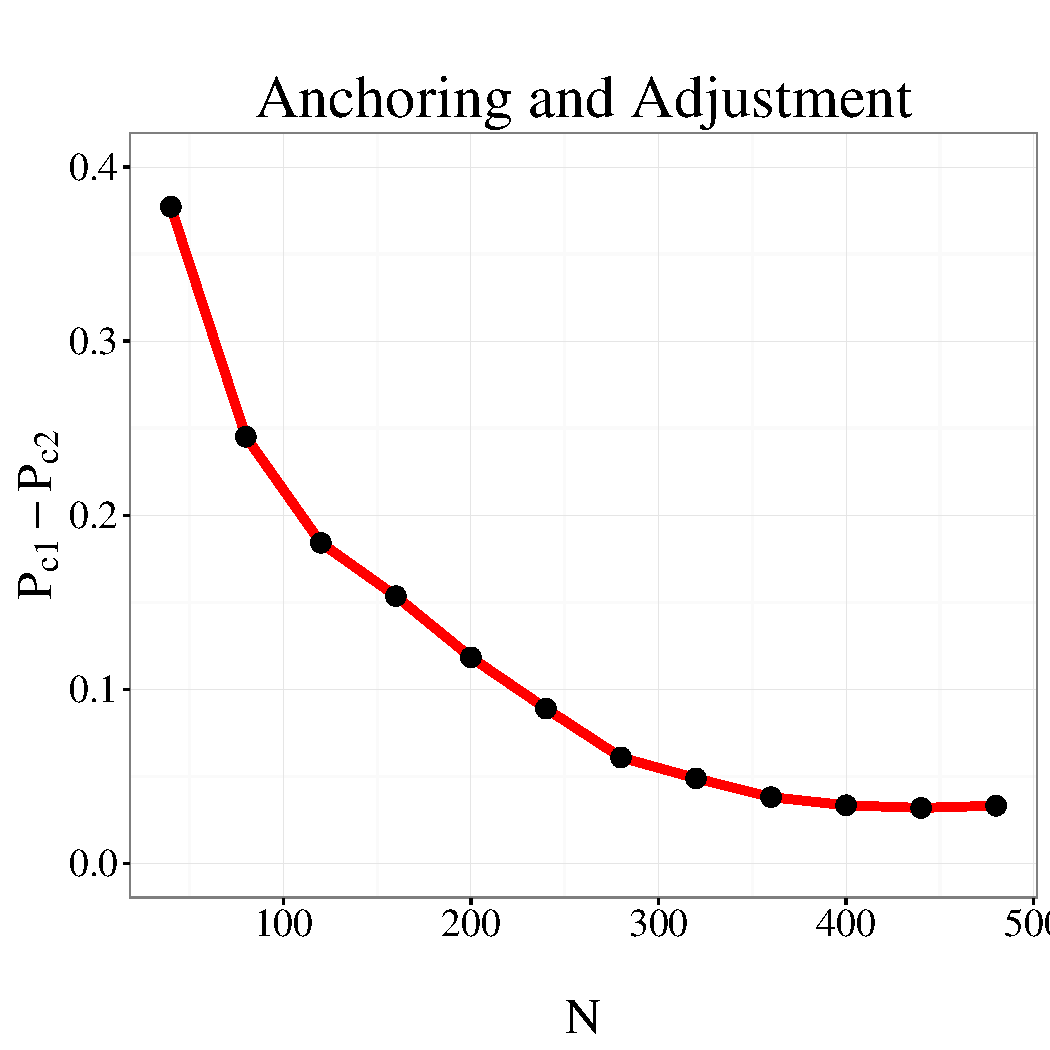
\includegraphics[scale = 0.5]{figures/anchoring.pdf}
\caption{\textbf{Anchoring and adjustment}. The y axis represents the difference in the probabilities of respiratory flu and stomach flu given the symptoms \textit{fever} and \textit{fatigue} as returned by two different chains that are initialized differently. The chains are initialized in the two different clusters, at hypotheses other than the focal hypotheses of \textit{respiratory} or \textit{stomach flu}. Before reaching convergence, the chain initialized in cluster 1 of respiratory diseases places higher probability on respiratory flu than the chain initialized in cluster 2 of gastrointestinal diseases. The net difference between the two chains diminishes as the number of samples increases.}
\label{fig:anch}
\end{figure}

\subsection{The crowd within}

Error in estimates of numerical quantities decrease when the estimates are averaged across individuals, a phenomenon known as the \emph{wisdom of crowds} \citep{surowiecki2005wisdom}. This is expected if the error in the estimate of one individual is statistically independent from the error of the others, such that averaging removes the noise. Any unbiased stochastic sampling algorithm replicates this result, because taking more samples gets one closer to the asymptotic regime, where the estimates are exact and the error tends to zero.

This error analysis was extended by \cite{vul08} to the effects of averaging across multiple estimates from a single individual. They found that averaging estimates reduced error---a phenomenon they named the \emph{crowd within}. However, they also found that this error reduction was less compared to the reduction obtained by averaging across individuals. One explanation for this observation is that the error in the estimates given by the same individual are not entirely independent. We propose that the dependence between multiple estimates arises from an autocorrelated stochastic sampling algorithm like MCMC. 
This effect is illustrated in Figure \ref{fig:asymptote}. We presented the following query to the model: Given symptoms are \emph{fever}, \emph{nausea} and \emph{fatigue}, what is the probability that these symptoms are caused by the presence of a respiratory disease rather than a gastrointestinal disease? We ran several chains ($N_c = 24$) initialized randomly in the space of all possible diseases, with each run generating the same number of samples ($N_s = 200$). Each chain is initialized at the last sample of the previous chain\footnote{We could also induce correlation between consecutive estimates by continuing the chain---i.e., carrying over the estimates from the first guess to the second one, instead of re-initializing. However, if we continue the chain, the second estimate is made with more samples and will always have a lower error on average than the first one. \cite{vul08} find this to not be the case empirically.}, for another $N_s$ steps and a new set of $N_c$ estimates are obtained, corresponding to the second guesses of the $N_c$ individuals. This process is continued until we have 7 estimates from each of the $N_c = 24$ participants. The samples are then averaged either within or across individuals (chains). We find results analogous to those in \cite{vul08}---the error of the responses monotonically declines with the number of samples, and the error reduction is greater when averaging across (compared to within) individuals.

\begin{figure}
\centering
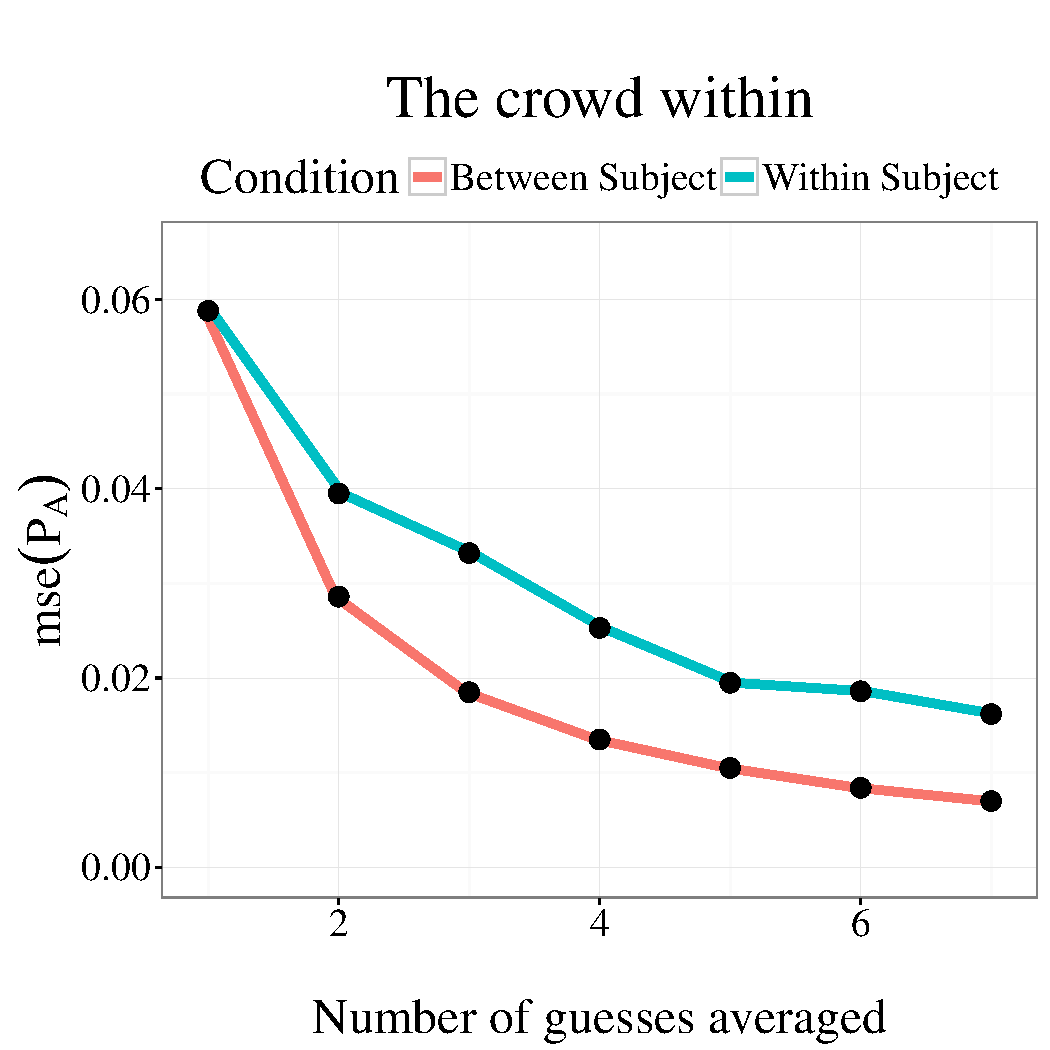
\includegraphics[scale = 0.5]{figures/error.pdf}
\caption{\textbf{The crowd within}. Errors in the MCMC estimates for the following query: Given the symptoms \emph{nausea} and \emph{shortness of breath}, what is the probability that these were caused by the presence of a respiratory disease? The estimates are averaged either over samples from the same individual (blue) or over samples from different individuals (red)}
\label{fig:asymptote}
\end{figure}

Our MCMC model can replicate this effect because it generates auto-correlated samples. The last sample from one estimate is where the chain for the next estimate is initialized. As the sampling process is auto-correlated, subsequent samples in the second chain (in the small sample size limit) are correlated to its initial sample. Similarly, earlier samples from the first chain are correlated to its last sample. Because the samples from the two chains are correlated via the common sample, the probability estimates they generated are correlated as well. This auto-correlation exists irrespective of proposal distribution because of the non-zero rejection probability, but is strengthened by locality in the proposals because this increases correlation.

\subsection{Summary of simulation results and comparison with importance sampling}

To highlight the distinctive predictions of MCMC, it is useful to compare it with other sampling algorithms that have been explored in the psychological literature. \emph{Importance sampling} also uses a proposal distribution $Q(h)$, but unlike MCMC it samples multiple hypotheses independently and in parallel. These samples are then weighted to obtain an approximation of the posterior:
\begin{align}
\hat{P}_N(h|d) = \frac{1}{N} \sum_{n=1}^N \mathbb{I}[h_n=d] w_n,
\end{align}
where $w_n$ is an ``importance weight'' for sample $n$ computed according to:
\begin{align}
w_n \propto \frac{P(h_n,d)}{Q(h_n)}.
\end{align}
Intuitively, the importance weight corrects for the fact that the importance sampler draws samples from the wrong distribution. \citet{shi10} have shown how this algorithm can be used to simulate human performance on a wide range of tasks. They also identified a correspondence between importance sampling and exemplar models, which have been widely applied in psychology. In related work, \citet{shi2009neural} demonstrated how importance sampling could be realized in a biologically plausible neural circuit \citep[see also][]{abbott13}.

Some of the effects we have replicated in this work could also be captured by an importance sampling algorithm with limited samples. \citet{Thomas2008} have proposed a model, HyGene, that is similar in spirit to an importance sampler with limited samples, with a memory driven proposal distribution that selects the hypotheses to be generated. HyGene explains subadditivity in terms of a failure to retrieve all the relevant hypotheses from memory due to stochastic noise in the retrieval process and limited working memory capacity.

The self-generation effect can to some extent be reproduced by importance sampling because prompting a hypothesis causes it to be sampled an extra time. So the probability of the focal space will be slightly larger if hypotheses in it are explicitly prompted (other-generated and presented to the participant) than if it they are generated without prompting (self-generated). However, Experiment 2 in \cite{conf} shows that in a situation where all the alternatives are specified, prompting specific hypotheses (as in the other-generated scenarios), does not result in a higher probability judgment than when these hypotheses are not prompted (as in the self-generated scenarios). The MCMC algorithm captures this finding because in a small hypothesis space, the Markov chain will visit all the hypotheses with the right frequency irrespective of initialization. By contrast, the importance sampler predicts a higher probability for other-generated hypotheses, contrary to the empirical finding.

This brings us to a key difference between importance sampling and MCMC: Importance sampling generates all hypotheses in parallel---the generation of new hypotheses has no dependence on hypotheses that have already been generated. Without this dependence, there is no interaction between the generation and evaluation processes. MCMC captures this dependence by sequentially generating hypotheses. Our model's explanation of the self-generation effect, superadditivity, the weak evidence effect and the dud alternative effect rests on this dependence. The Markov chain can get stuck (at least temporarily) by rejecting proposals, thus generating fewer alternatives. If, on the other hand, the current hypothesis has low probability, more alternatives are generated and the probability estimate of the focal space is reduced.

The importance sampler does not produce these effects, because its mechanism for generating new hypotheses is independent of the probability of the current one. If anything, prompting a hypothesis within the focal space, no matter how atypical, causes it to be sampled, \textit{increasing} the importance sampler's estimate for the probability of the focal space, contradicting superadditivity.

Another key difference between MCMC and importance sampling is that MCMC generates correlated samples, whereas consecutive samples from an importance sampler are totally independent. This prevents the importance sampler from reproducing the effects in Table \ref{tab:biases} that rely on correlated sampling, such as the anchoring effect and the crowd within.

It is also valuable to contrast MCMC with anchoring and adjustment schemes that involve incremental changes to a numerical estimate in the direction of the target value. Although MCMC produces autocorrelation of samples, it does not require changes to be incremental; MCMC allows the proposal distribution to be non-local. In fact, substantial evidence suggests that some of these changes can be quite dramatic, as in perceptual multistability \citep{Gershman2012} and insight problem-solving \citep{sternberg95}. 

\section{Overview of experiments}

We now turn to novel experimental tests of our theory. As discussed in the Introduction, the primary impetus for considering rational process models based on approximate inference is that inference in many real-world problems is computationally intractable. However, studying complex inference problems experimentally is challenging because it becomes harder to control participants' knowledge about the generative model. In the case of medical diagnosis, we can rely on the extensive training of clinicians, but it is unclear whether conclusions from these studies are generalizable to non-expert populations. Thus, for our experiments we sought a more naturalistic inference problem.

One domain in which humans have rich, quantifiable knowledge is scene perception and understanding. Extensive research suggests that the visual system encodes information about natural scene statistics \citep{barlow2001exploitation,simoncelli2001natural}.
%start%%%%%%%%%%%%%%%%%%%%%%%%%%%%%%
%%%%%%%%%%%%%%%%%%%%%%%%%%%%%%%
Although these low-level scene statistics like the distribution of oriented edges are not consciously accessible, statistics at the level of objects, for example object co-occurrence statistics in natural scenes studied in \citet{greene13}, can be used to inform a generative model that can act as a proxy for one aspect of human scene understanding. We can then leverage such models to test theories of hypothesis generation in this domain.

Specifically, \citet{greene13} provides a database of natural scenes with hand-labeled objects. We fit the latent Dirichlet allocation (LDA) model \citep{lda} to this dataset, allowing us to capture the distribution of co-occurrences of different objects in terms of latent ``topics'' (distributions over objects). Each scene is modeled as a probabilistic mixture of topics. The LDA model captures the fact that microwaves are likely to co-occur with toasters, and cars are likely to co-occur with mailboxes. The marginal distribution of objects provides a natural empirical prior over objects. We do not fit any free parameters to the dataset; all hyperparameters are set to the values described in \citet{lda}.

%End%%%%%%%%%%%%%%%%%%%%%%%%%%%%%%

For our purposes, the important point is that we can use our model to compute conditional probabilities over hidden objects in a scene, given a set of observed objects. Formally, let $h \in \mathcal{H}$ denote a hypothesis about $k$ hidden objects in a scene, among all such possible hypotheses $\mathcal{H}$. Given a set of observed objects $d$, the inference problem is to compute the conditional probability $P(h \in H|d)$ that $h$ is in some set $H \subset \mathcal{H}$ (e.g., hypotheses in which at least one of the hidden objects is an electrical appliance, or hypotheses in which the name of at least one of the hidden objects starts with a particular letter). This conditional probability can be approximated using MCMC in the hypothesis space.

In our experiments, we present participants with a set of observed objects, and ask them to estimate the probability that the hidden objects belong to some subset of possible objects. By manipulating the query, we attempt to alter the initialization of participants' mental sampling algorithm, allowing us to quantitatively test some of the predictions of our model. 

Due to the relative complexity of this domain (compared to the simplified fictitious disease-symptom domain we have used so far for illustrative purposes), we refrain from making claims about the structure of proposal locality here and only test the predictions of our model that are immune to the choice of proposal distribution. Specifically, we focus on subadditivity and superadditivity.

%Considering these are natural images and have been labeled by people, we expect that the results from the topic model provide a fair approximation of people's generative model for scenes. This then provides access to the probability distribution over topics given observed objects, as well as the probability distribution over objects given a topic. Therefore, given the presence of some object in a natural scene, we can simulate probability judgments over the presence of other objects in the same scene. More precisely - the topic model can give us the joint probability of the presence of any two objects. We can generate the posterior probability over all other objects (the unknown variables, Y), given the presence of a specific object (the data, say X) by marginalizing this joint distribution over Y. The posterior probability  $P_{X} (Y)$ over all objects Y (except X, the one that is already known to be present) is approximated by Monte Carlo sampling as before. The probability of the presence of any Y, conditioned on the presence of X is then given by Equation~\label{eq:conv}.


% An important point to note is that this value does not affect any of our qualitative results because the function in Equation \ref{eq:conv} is monotonic in $P_X(Y)$ irrespective of the value of $k$. So the prediction that some probability judgments will be greater or less than another one is unaffected by the specific value of $k$.

\section{Experiment 1: Manipulating question framing}

Our first prediction is the occurrence of both superadditivity and subadditivity in the same domain. The key factor is the typicality of the examples prompted by the unpacked query. We predict that if the query prompts typical examples from the focal space, probability judgments of that focal space will be higher than in the packed condition where no hypotheses are prompted (subadditivity). By contrast, if the question prompts atypical examples from the focal space, probability judgments of that focal space will be lower than in the packed condition where no hypotheses are prompted (superadditivity).

Using LDA as the probabilistic model, the data consist of visible objects in a scene, and the hypotheses are hidden objects. The focal space of hypotheses is given by a query such as \emph{all objects starting with `c'}. The focal space was unpacked into several either highly probable (typical) examples or highly improbable (atypical) examples, as well as a catch-all hypothesis. In the packed condition, the focal space is queried without any unpacked examples.

\subsubsection{Participants}
59 participants (26 females, mean age=35.76, SD=11.63) were recruited via Amazon's Mechanical Turk and received \$1 for their participation plus a performance-dependent bonus.

\subsubsection{Materials and procedure}
Participants were asked to imagine playing a game with a friend in which the friend specifies an object in a scene that they cannot see themselves. The task is to estimate the probability of certain sets of other objects in the same scene. For example, the friend could specify ``pillow''. In the unpacked condition, participants were then asked to estimate the conditional probability of a focal space presented as a few examples and a catch-all hypothesis (e.g., ``an armchair, an apple, an alarm clock or any other object starting with an A''). In the packed condition, the query did not contain any examples.


\begin{table}[htbp]
% \setstretch{0.5\baselineskip}
\caption{Queries in Experiment 1. The letter determines the focal space (e.g., all objects beginning with A), conditioned on the cue object. Typical and atypical unpackings are shown for each focal space.}
\label{tab:scenarios}

  \begin{center} 
\begin{tabular}{m{.12\textwidth}  p{.08\textwidth} >{\raggedright}p{.32\textwidth} >{\raggedright}p{.36\textwidth}}
  \toprule
\bf{Cue object} & \bf{Letter} & \bf{Unpacked-typical} & \bf{Unpacked-atypical}\tabularnewline
\midrule
Pillow & A & armchair, alarm clock, apple & arch, airplane, artichokes\tabularnewline
Rug & B & book, bouquet, bed & bird, buffalo, bicycle\tabularnewline
Table & C & chair, computer, curtain & cannon, cow, canoe\tabularnewline
Telephone & D & display case, dresser, desk & drinking fountain, dryer, dome\tabularnewline
Computer & E & envelope,electrical outlet, end table & eggplant, electric mixer, elevator door\tabularnewline
Armchair & F & fireplace, filing cabinet, fan& fire hydrant, fountain, fish tank\tabularnewline
Stove & L & light, lemon, ladle& leavers, ladder, lichen\tabularnewline
Chair & P & painting, plant, printer& porch, pie, platform\tabularnewline
Bed & R & rug, remote control, radio & railroad, recycling bins, rolling pin\tabularnewline
Kettle & S & stove, shelves, soap& suitcase, shoe, scanner\tabularnewline
Sink & T & table, towel, toilet & trumpet, toll gate, trunk\tabularnewline
Lamp & W & window, wardrobe, wine rack & wheelbarrow, water fountain, windmill\tabularnewline
\bottomrule

\end{tabular}
\end{center}
\end{table}



Each participant responded to one query for each of 9 different scenarios shown in Table~\ref{tab:scenarios}, with 3 unpacked-atypical, 3 unpacked-typical, and 3 packed questions. We randomized the order of the scenarios as well as the assignment of scenarios to condition for each participant.

On every trial, participants first saw the cue object, followed by a hypothesis (either packed, unpacked-typical or unpacked-atypical). Participants had 20 seconds to estimate the probability of the hypothesis on a scale from 0 (not at all likely) to 100 (certain). For every timely response per trial they gained an additional reward of \$0.1. A screenshot of the experiment is shown in Figure~\ref{fig:screenshot}.

\begin{figure}[ht!]
\centering
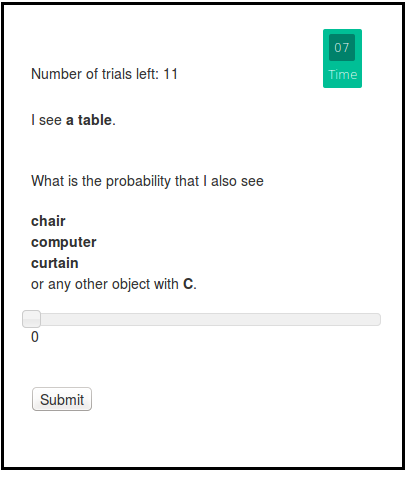
\includegraphics[scale=0.9]{figures/screenshot.png}
\caption{\textbf{Experimental setup}. Participants were asked to estimate the conditional probability using a slider bar within a 20-second time limit.}
\label{fig:screenshot}
\end{figure}

\subsubsection{Model fitting}
Our model has two free parameters: the number of hidden objects in the scene ($k$) and the number of samples ($N$). These parameters were fit to the behavioral data from both Experiment 1 and Experiment 2 combined, using a coarse grid search to optimize the mean-squared error between the mean experimental probability estimates and the probability estimates from the model.
%start2
 This estimate was used to generate confidence intervals.
The value of $k$ that best fit the data was $k=6$ with negligible uncertainty, and the number of samples $N = 230$ with a $95\%$ confidence interval $[191, 269]$. 
%end
This value of $k$ is in the same ballpark as values found for average number of uniquely labeled objects in natural scenes from data collected in \cite{greene13}. This value for $N$ as the number of samples is higher than numbers found in some previous work like \cite{Vul2014} etc, but it is important to note that each unique hypothesis can appear several times in the sample set. So even if the number of samples is larger than in previous studies, the number of unique hypotheses is comparable.

%********************************************
%********************************************
The details of the proposal distribution could also influence the individual and relative magnitudes of the observed subadditivity and superadditivity effects, and perhaps different parameters for $N$ and $k$. Instead of making strong assumptions about locality in this particular hypothesis space, we use a uniform proposal distribution. 
%********************************************

\subsubsection{Results and discussion}
We compared the mean probability judgments for each condition (Figure~\ref{fig:results1}). Consistent with our hypothesis, we found subadditivity in the unpacked-typical condition, with significantly higher probability estimates compared to the control condition $[t(58)= 4.53, p<0.01]$, and superadditivity in the unpacked-atypical condition, with significantly lower probability estimates compared to the control condition $[t(58)= -4.97, p<0.01]$. This pattern of results was captured by our MCMC model.

\begin{figure}[ht!]
\centering
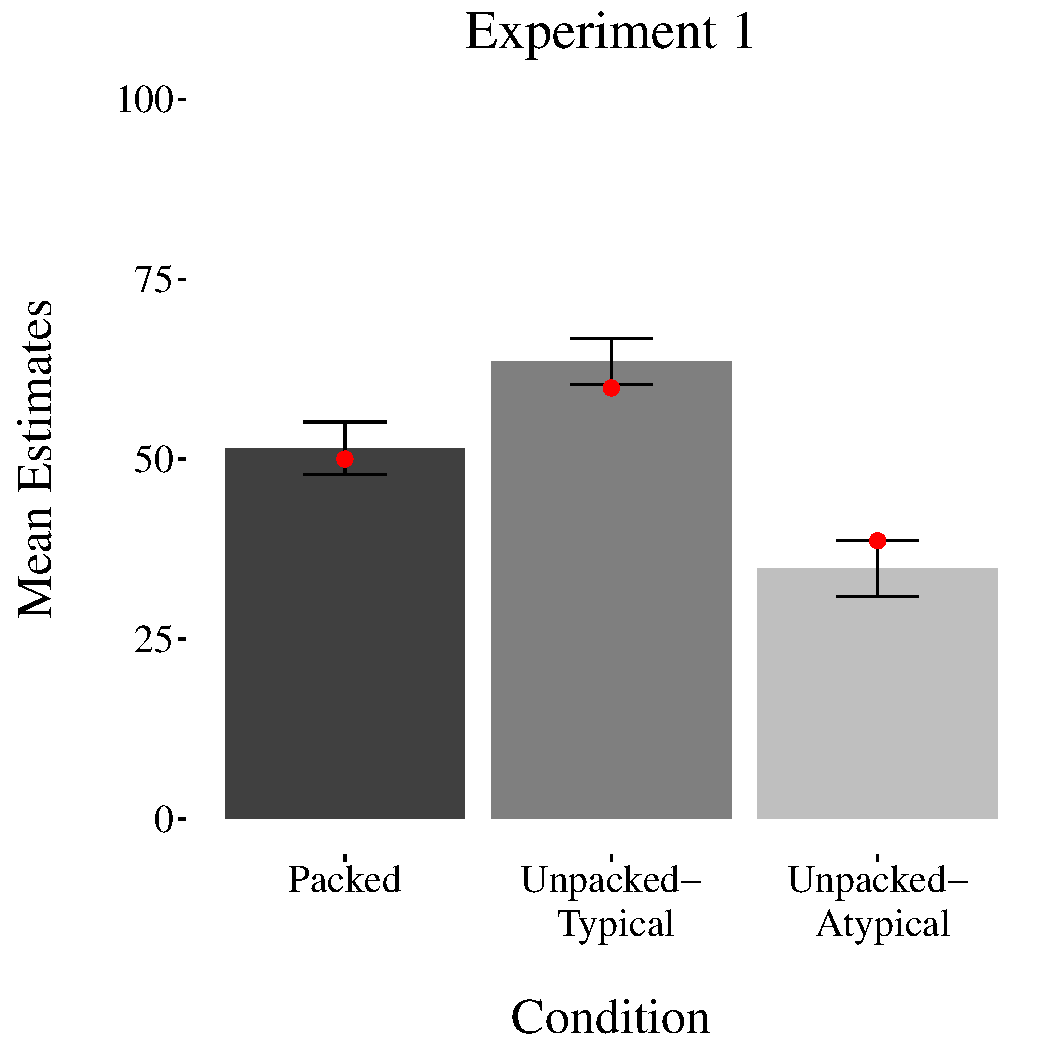
\includegraphics[scale=0.5]{figures/estimates.pdf}
\caption{\textbf{Experiment 1 results}. Mean probability estimates for each condition. Error bars represent the 95\% confidence interval of the mean. Red dots show estimates from the MCMC model with 230 samples, assuming 6 hidden objects in the scene.}
\label{fig:results1}
\end{figure}

Our results confirm the prediction that subadditivity and superadditivity will occur within the same paradigm, depending on the typicality of unpacking. A related result was reported by \cite{super}, who found subadditivity only when the definition of the focal space was fuzzy and typical unpacking may have led to the consideration of a larger focal space. We consider this study in more detail in the General Discussion.

\section{Experiment 2: Manipulating the cue}

In Experiment 1, we demonstrated that the typicality of unpacked examples has a powerful effect on biases in probability estimation. In Experiment 2, we provide converging evidence by showing that different biases can be induced for the same unpacked examples by changing the cue object.

Typicality depends on an interaction between the cue and the examples: in the presence of a road, a crosswalk is typical and a coffee-maker is atypical, but the opposite is true in the presence of a sink. Our model predicts that subadditivity will occur when unpacked examples are typical for a given cue object, whereas superadditivity will occur when the same examples are atypical for a different cue object.

%This gives us scenarios where the unpacking causing subadditivity for cue object 1 produces superadditivity for cue object 2 and vice versa. The resulting scenarios are shown in Table~\ref{tab:scenarios2} below. The examples that showed detectable effects in the MCMC model after a chain length of 100 were retained.

%we could only choose query objects that were largely typical in the presence of one cue object but became largely atypical in the presence of a different cue object. So none of the objects we considered could have a very low (or a very high) prior - because then they would be largely atypical (or typical) independent of cue-word. As all the query objects in this experiment were restricted to having an intermediate prior, they are neither \textit{very} typical nor \textit{very} atypical for either cue-word, resulting in weaker effects. Further, as generating these kind of scenarios was generally more difficult, we also had to restrict the unpacking to two objects instead of three as in the experiment before. We therefore expected all of the effects, to be less pronounced than before.

\subsubsection{Participants}
180 participants (84 females, mean age= 34.25, SD=11.16) were recruited via Amazon's Mechanical Turk web service and received \$0.5 for their participation plus a performance-dependent bonus.

\subsubsection{Materials and procedure}
The experimental procedure was identical to Experiment 1, except for the choice of scenarios (Table~\ref{tab:scenarios2}). Each participant responded to one unpacked-typical, one unpacked-atypical and one packed scenario in random order.

\begin{table}[htbp]
\caption{Queries in Experiment 2. The letter determines the focal space (e.g., all objects beginning with A), conditioned on the cue object. Conditioned on cue object 1, unpacking 1 is predicted to cause subadditivity and unpacking 2 is predicted to cause superadditivity. These predictions reverse for cue object 2.}
\label{tab:scenarios2}
  \begin{center} 
\begin{tabular}{p{.14\textwidth} p{.14\textwidth} p{.05\textwidth} >{\raggedright}p{.24\textwidth} >{\raggedright}p{.25\textwidth}}
  \toprule
\bf{Cue object 1}&\bf{Cue object 2}&\bf{Letter}&\bf{Unpacking 1} &\bf{Unpacking 2}\tabularnewline
\midrule
Pillow & Faucet & B & bed skirt, bedspread\ & bucket, bread\tabularnewline
Road & Sink & C & cabin, crosswalk & cup, coffee maker\tabularnewline
Cabinet & Road & T & toothpaste, tray & terrace, tunnel\tabularnewline
\bottomrule
\end{tabular}
\end{center}
\end{table}

\begin{figure}
\centering
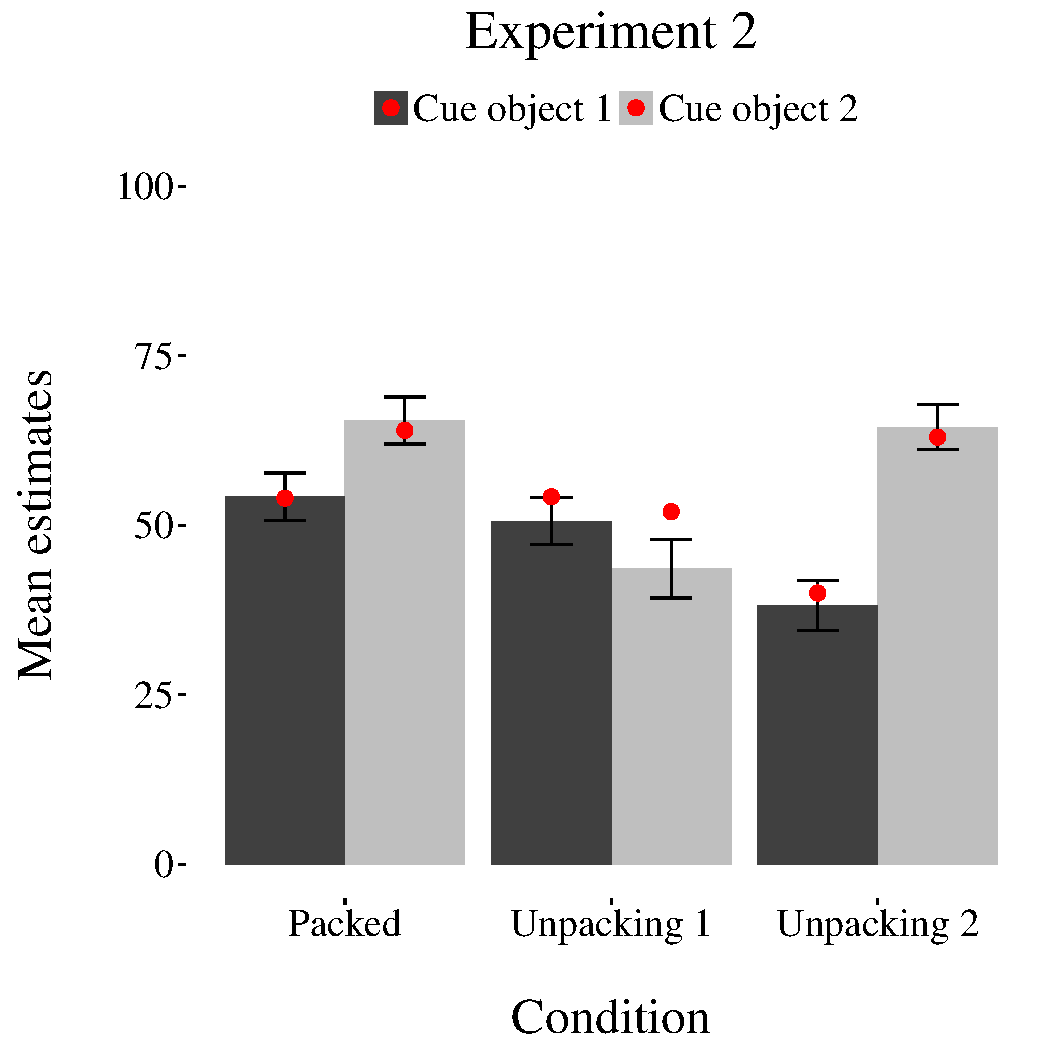
\includegraphics[scale=0.5]{figures/estimate2new.pdf}
\caption{\textbf{Experiment 2 results}. Mean probability estimates for each condition. Error bars represent the 95\% confidence interval of the mean. Red dots show estimates from the MCMC model with 230 samples, assuming 6 hidden objects in the scene. Unpacking 1 is typical for cue object 1 and atypical for cue object 2; unpacking 2 is typical for cue object 2 and atypical for cue object 1.}
\label{fig:results2}
\end{figure}

\subsubsection{Results and discussion}
As shown in Figure~\ref{fig:results2}, we observed a superadditivity effect: probability estimates were significantly higher in the packed condition compared to the atypical unpacking for both cue object 1 $[t(165)=3.31, p<0.01]$ and cue object 2 $[t(162)=4.31, p<0.01]$. We did not observe a subadditivity effect for either cue object 1 [$t(171)=0.73, p>0.05]$ or cue object 2 $[t(168)=0.08, p>0.05]$. Importantly, we found a significant interaction between the cue-object and the unpacking of the objects $[F(498, 2)=12.69, p<0.001]$. In particular, when conditioning on cue object 2, using ``Unpacking 1'' (see Table~\ref{tab:scenarios2}) leads to significantly lower estimates than using ``Unpacking 2'' $[t(251)=2.52 , p<0.01]$. Additionally, when conditioning on cue object 1, using ``Unpacking 2'' produces significantly lower estimates than using ``Unpacking 1''; $[t(165)=-3.31, p<0.001]$. These results show that typicality of the unpackings and, by proxy the sub- and super-additive effects, crucially depend on the conditioned cue object.

% unpacking the first cue objects via Unpacking 1 lead to estimates that are not significantly different from the packed estimates $[t(171)=0.74, p>0.05]$, while unpacking it via ``Unpacking 2'' produces significantly lower estimates $[t(165)=-3.31, p<0.001]$. These results seem to 

Our fitted model matches the experimental data well ($r=0.96$, $p<0.001$), only slightly underestimating the superadditive effect with cue object 2 and unpacking 1. We can conclude from the fact that this cue-dependent swap can be even partially carried out---for example, the superadditivity effect certainly does get swapped---indicates that these effects are not modulated solely by the prior typicality or inherent availability of the unpacked examples. The same unpacking that induces superadditivity in the presence of one cue object, does not induce it in the presence of the second cue object. Furthermore, a new unpacking can be chosen such that it induces superadditivity in the presence of the second cue object but not in the presence of the first. These results support a sampling process that is modulated by the cue objects, i.e. the observed data.

%In Experiment 1, we found that while the subadditivity effect was weaker than superadditivity, it was nonetheless still captured. For this experiment, only superadditivity is observable. We attribute the mismatch between our results from experiment 1 and experiment 2 to the fact that the effects are expected to have been weaker in experiment 2 and, given that subadditivity is already a weaker effect than superadditivity, may already have died away in the 20 second window provided. The model supports this explanation---its predictions in Fig. \ref{fig:results2} show that for a chain length of 230 (the best fit chain length for both experiments combined) the effect for subadditivity is almost totally gone, i.e. the probability estimate from the typically unpacked scenario is comparable in value to the estimate from the packed hypothesis.


%\cite{super} found similar results for queries on ``well-defined categories''. However, we believe the the reason that both these experiments observe superadditivity and not subadditivity, are different. We expound on this in the General Discussion.
\section{Experiment 3: The effect of time pressure}

A key prediction of our model is that the strength of subadditivity and superadditivity will decrease with the number of sampled hypotheses, as the chain approaches its stationary distribution. To test this prediction, we repeated Experiment 1, but reduced the time limit and incentivized participants to respond more quickly. We predicted that these changes would lead to stronger subadditivity and superadditivity effects.

\subsubsection{Participants}
62 participants (34 females, mean age= 25.65, SD=12.36) were recruited via Amazon's Mechanical Turk web service and received \$0.5 for their participation plus a performance-dependent bonus.

\subsubsection{Materials and procedure}
Materials were the same as in Experiment 1. However, in this experiment participants had less time available per trial (5 seconds) and were asked to respond as quickly as possible. Participants were paid a baseline amount for their participation of \$0.5. Additionally, they were incentivized to respond quickly: they could gain more money the faster they responded on each trial (up to \$0.1 per trial) and gained an additional \$0.1 for every on time response per trial overall.

\subsubsection{Results and Discussion}

The mean estimates for the different conditions are shown in Figure~\ref{fig:resultstime}. Replicating the results of Experiment 1, the estimates for the unpacked-atypical condition were significantly lower than for the packed condition $[t(57)=-4.8183, p<0.01]$, and the estimates for the unpacked-typical condition were significantly higher than for the packed condition $[t(57)=4.76, p<0.01]$. 
%start2
Our hypothesis generation model fits the data well with parameter values $K = 3$ with negligible uncertainty and $N = 170$ with $95\%$ confidence interval $[94, 246]$. We see that the best fit number of samples is substantially lower than that found in Experiment 1 ($N = 230$, with $95\%$ confidence interval $[191, 269]$).
%end2
The number of hidden objects $K$ is also lower. These parameter estimates are consistent with the idea that time pressure results in fewer generated samples and fewer objects under consideration. 
%ES2: Ishita, can you add something about how meaningful the different estimates are here? Just say something about how they produce a distinct relative effect for example.

\begin{figure}[ht!]
\centering
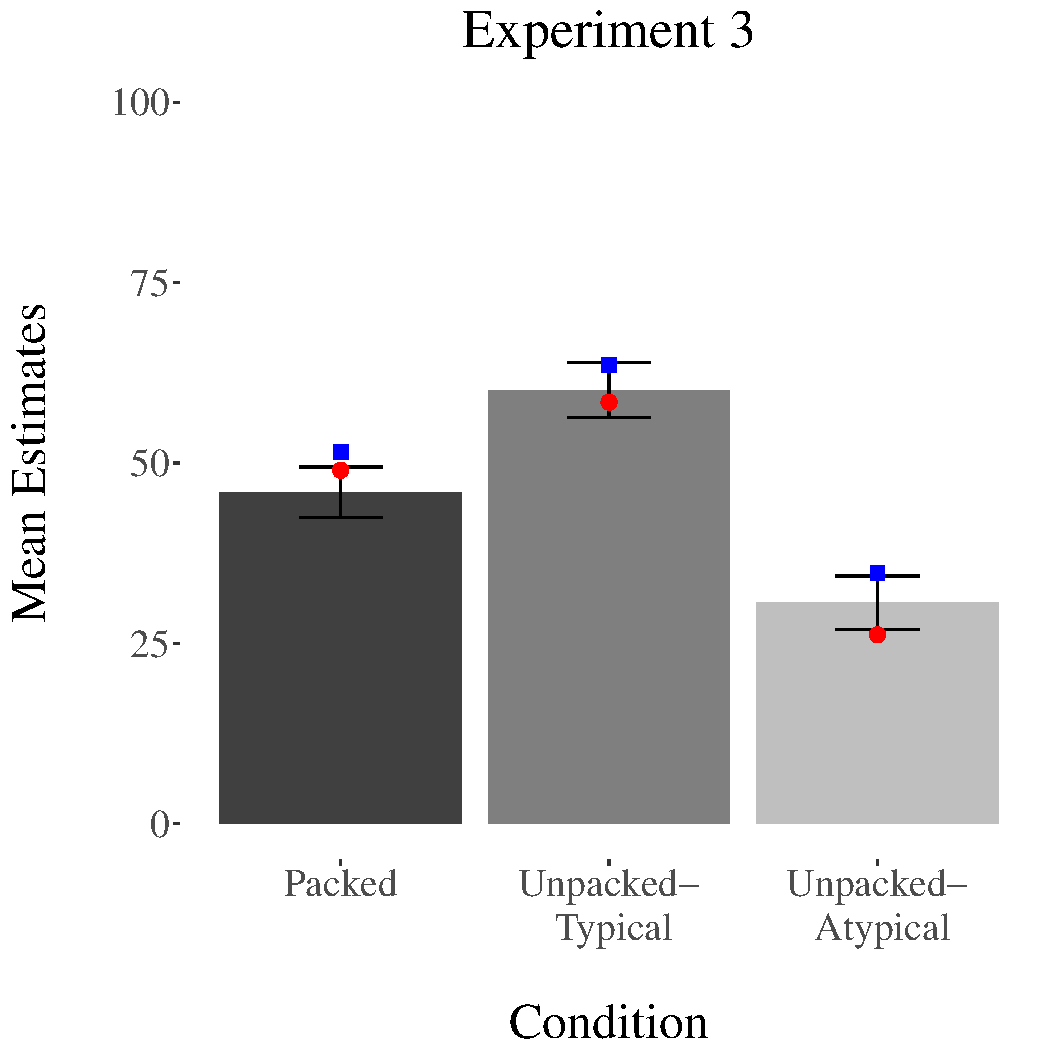
\includegraphics[scale=0.5]{figures/estimates3.pdf}
\caption{\textbf{Experiment 3 results}. Mean probability estimates for each condition. Error bars represent the 95\% confidence interval of the mean. Red dots show estimates from the MCMC model with 170 samples, assuming 3 hidden objects in the scene. Blue squares show means estimates of Experiment 1.}
\label{fig:resultstime}
\end{figure}

Next, we performed a median split based on the overall reaction times and thereby classified trials into slow and fast trials. The slow and fast trials were separately fit using the same value of $K$ from the overall responses and adjusting $N$.
%start2
We see that the data from the fast trials are better fit with a lower $N$ ($N = 150$, with $95\%$ confidence interval $[98, 202]$) than the slow trials ($N = 190$, with $95\%$ confidence interval $[125, 255]$). The estimates for the slow trials have a high overlap with the estimates from Experiment 1 ($N = 230$, with $95\%$ confidence interval $[191, 269]$). However, the intervals for the fast response and the one from Experiment 1 have a small overlap of $\sim 10$ steps. 
%end2
The results are shown in Figure~\ref{fig:medsplitexp3}. We then performed an ANOVA, regressing the median time (fast or slow response), condition (packed, typically unpacked and atypically unpacked hypothesis) onto participants' probability estimates, where responses were nested within participants. Condition was a significant predictor of participants' responses ($\chi^2(1)=157.8$, $p<0.001$). The time variable alone was not a significant predictor of participants' responses ($\chi^2(1)=3.9$, $p=0.05$). This is expected since the subadditivity and superadditivity effects go in opposite directions. The interaction between time and condition was significant ($\chi(1)=37.03$, $p<0.01$) indicating that the time variable influences the estimates depending on condition. Further assessing this difference between the interactions again using a nested ANOVA showed that faster responses produced greater subadditivity effect as compared to slow responses ($t(248)=-2.1602$, $p<0.05$). The difference in the superadditivity effect however was not significant ($t(213)= 0.78$, $p=0.4$).
%ES:New effect comparison:
Comparing the sub- and superadditivity effects of Experiment 3 to the effects of Experiment 1, we found that they were relatively similar overall ($t(453)=-1.353$,$p>0.1$). However, comparing only the fast responses from Experiment 3 to the results of Experiment 1, we found an increased subadditivity effect ($t(102)=-2.46$, $p<0.05$) but a similar superadditivity effect ($t(104)=-0.71$, $p=0.48$).
%start2
This is in agreement with the model fits.
%end2

\begin{figure}[ht!]
\centering
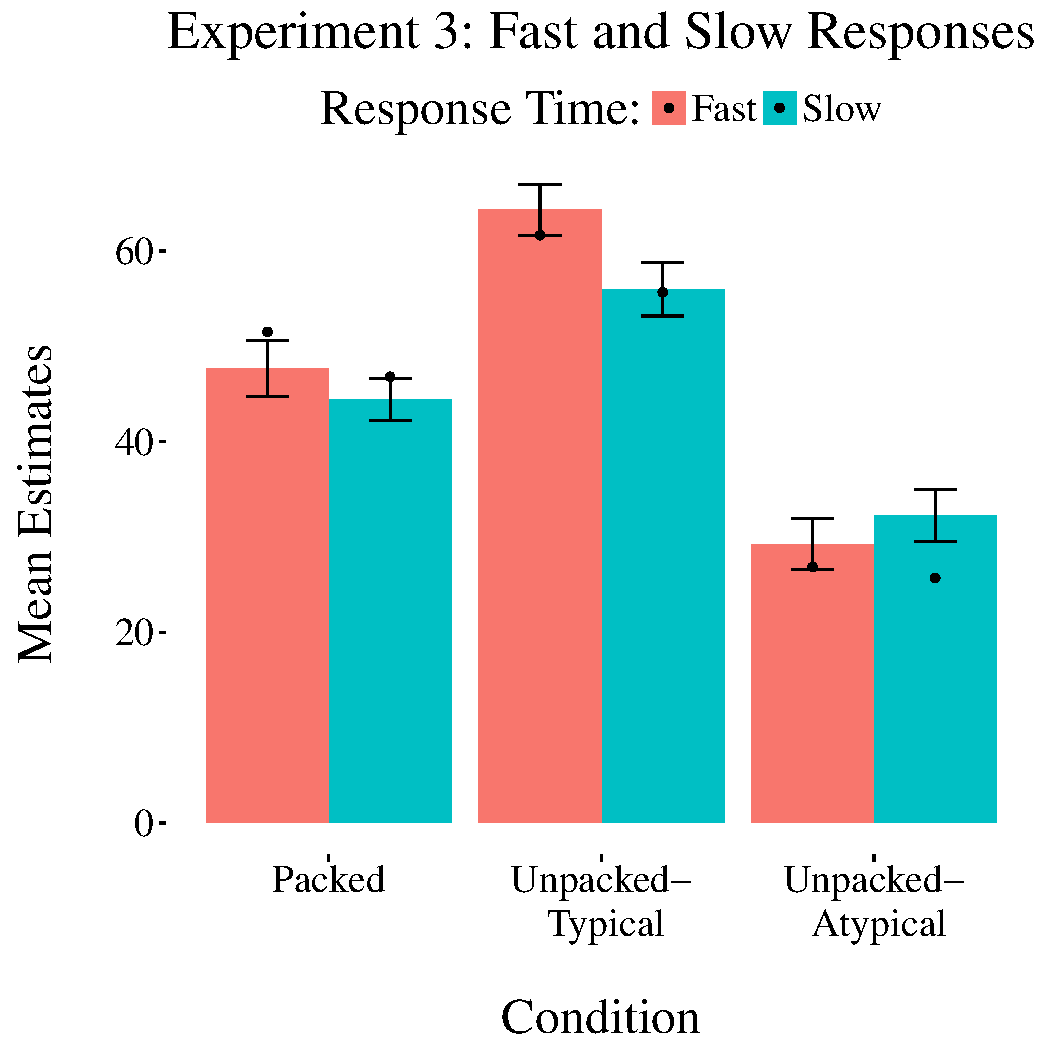
\includegraphics[scale=0.4]{figures/mediantimeexp3.pdf}
\caption{\textbf{Experiment 3 results: response time analysis}. Mean probability estimates for each condition divided into fast and slow trials based on a median split of the response times. Error bars represent the 95\% confidence interval of the mean. Dots represent the model fits with model parameters $K = 3$, and $N = 150$ for the fast trials and $N = 190$ for slow trials.}
\label{fig:medsplitexp3}
\end{figure}

%Analyzing the average effect per participant, that is how much higher every participant's response in a typically unpacked scenario was compared to the average of the same scenario presented as a packed hypothesis over all participants and, vice versa, lower for atypically unpacked scenarios, we found that this measure of effect-size correlates negatively with log-time ($r=-0.16$, $p<0.01$) and also negatively with the median-thresholded time ($r=-0.11$, $p<0.01$). This again shows that the overall effect seems to get stronger with shorter time i.e. as --hypothetically-- fewer samples are generated.

%We expect that this reflects the relative difficulty of the queries in this experiment compared to Experiment 1; the more difficult the question, the smaller the number of hidden objects considered by the participants. The parameters are manifested in the model predictions as follows: $K$ determines the absolute value of the judgments across all conditions (high K implies higher probability judgments overall), and $N$ determines the relative values of the judgments between conditions (lower N implies higher differences in the judgments between conditions). 
% and that this effect --as predicted by our model-- might be more easily detectable for the superadditivity than for the subadditivity condition.

%EXPERIMENT 4
\section{Experiment 4: The effect of cognitive load}

In our final experiment, we explored the possibility that cognitive load will reduce the number of samples, under the assumption that load consumes resources necessary for hypothesis generation. Therefore, we repeated Experiment 1, but put participants under cognitive load while responding to the packed or unpacked queries. We predicted that subadditivity and superadditivity effects should become stronger under cognitive load. In addition, the effects should again depend on participants' response time, such that faster trials are expected to produce larger effects.

\subsection{Participants}
69 participants (28 females, mean age= 32.17, SD=7.64) were recruited via Amazon's Mechanical Turk web service and received \$0.5 for their participation plus a bonus of \$0.1 for every question they answered on time and \$0.1 for every time they remembered whether or not an item shown after the question had a appeared within a sequence before the target question correctly.

\subsection{Materials and Procedure}
Materials were the same as in Experiment 1 and 3. Additionally, participants were put under cognitive load while performing the probability estimation task. On each trial, participants again first saw the cue object. Once they clicked ``Next'', a sequence of three random digits appeared, each remaining on the screen for 1 second before disappearing after which the next digit appeared. Participants were asked to remember these digits. Immediately afterwards, participants were asked to judge the probability of a hypothesis that could be either packed or unpacked (same as in Experiment 1). They were then shown another digit and had to indicate whether or not that digit had occurred within the sequence they had just been shown.

\begin{figure}[ht!]
\centering
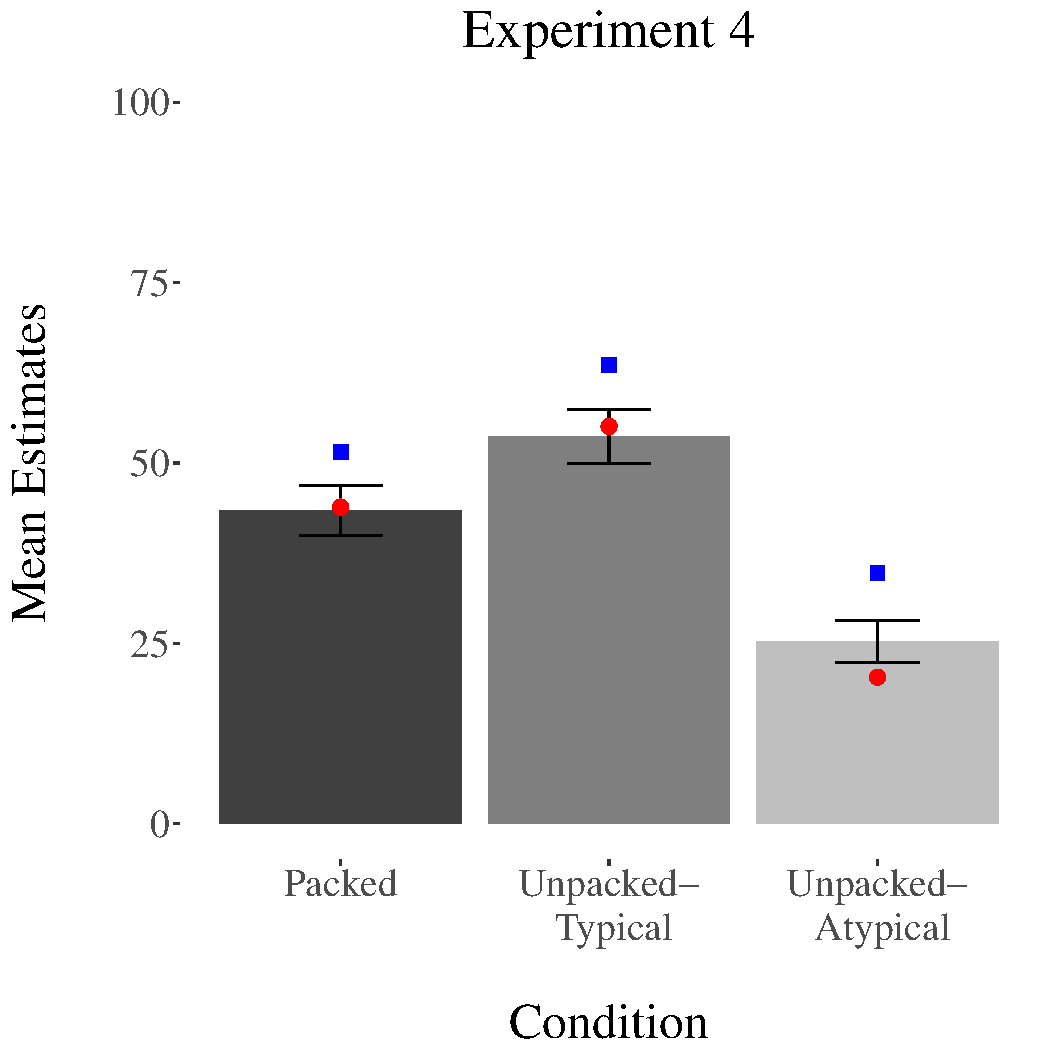
\includegraphics[scale=0.5]{figures/estimates4.pdf}
\caption{\textbf{Experiment 4 results}. Mean probability estimates for each condition when participants are put under cognitive load. Error bars represent the 95\% confidence interval of the mean. Red dots show estimates from the MCMC model with 110 samples, assuming 2 hidden objects in the scene. Blue squares show means estimates of Experiment 1.}
\label{fig:results4}
\end{figure}

\subsection{Results and Discussion}

The mean probability estimates for each condition are shown in Figure~\ref{fig:results4}. Again replicating Experiment 1, the estimates for the unpacked-atypical condition were significantly lower than for the packed condition $[t(68)=-7.31, p<0.01]$, and the estimates for the unpacked-typical condition were significantly higher than for the packed condition $[t(68)= 4.18, p<0.01]$. 
%start2
The model fits the data well with parameter values $K = 2$ and $N = 110$ with $95\%$ confidence interval of $[74, 146]$. We see again that the best fit number of samples is substantially lower than that found in Experiment 1 ($N = 230$, with $95\%$ confidence interval $[191, 269]$), with no overlap in the confidence intervals. 
%end2
The number of hidden objects $K$ is also lower. Additionally, the cognitive load manipulation increased the effect of superadditivity (packed-atypical condition) as compared to Experiment 1 $[t(58)=10.38, p<0.001]$, but was not significantly different from Experiment 1 for the subadditivity effect (packed-typical condition) $[t(58)=-1.9, p>0.05]$. 

%ES2: I think we could add something like the summary sentence below making clear what we have and haven't found. We can just be honest and say that not all but some manipulations worked, I think that's fine. I need your input though on stating something more explicit about what other sampling approaches would have predicted here.

%In summary, ....

\section{General Discussion}

We have presented a rational process model of inference in complex hypothesis spaces. The main idea is to recast hypothesis generation as a Markov chain stochastically traversing the hypothesis space, such that hypotheses are visited with a long-run frequency proportional to their probability. Our simulations demonstrated that this model reproduces many observed biases in human hypothesis generation. Finally, we confirmed in four experiments the model's prediction that subadditivity and superadditivity depend critically on the typicality of unpacked examples and that the superadditivity effect increases under time pressure and cognitive load.

Our work extends a line of research on using rational process models to understand cognitive biases. Most prominently, \citet{Thomas2008} have attempted in their HyGene model to explain a wide range of hypothesis generation phenomena by assuming that Bayesian inference operates over a small subset of hypotheses drawn from memory. We follow a similar line of reasoning, but depart in the assumption that hypotheses may be generated \emph{de novo} through stochastic exploration of the hypothesis space. This assumption is important for understanding how humans can generate hypotheses in complex combinatorial spaces where it is impossible to store all relevant hypotheses in memory.

Prior studies suggest that---when averaged over long time periods or across individuals---probability estimates converge roughly to the Bayesian ideal \citep{Vul2014}. Like other models based on Monte Carlo methods \citep[e.g.,][]{multistability,lieder2017empirical,lieder2017anchoring,shi10}, our model predicts exact Bayesian inference in the limit of large sample sizes. However, cognitively bounded agents are expected to be \emph{computationally rational} \citep{Gershman2015}: sampling takes time and effort, and hence the optimal sampling strategy will tend to generate relatively few hypotheses \citep{Vul2014}. 

Our model recreates several cognitive biases exhibited by humans: subadditivity, superadditivity, anchoring and adjustment, weaker confidence in self-generated hypotheses, the crowd within, and the dud alternative and weak evidence effects. While some of these biases have been accounted for by other models, ours is the first unified rational process account. Table \ref{tab:compare} provides a systematic comparison of which phenomena are accounted for by different models.

Our simulation results rest on two key features of the model, that are not captured by parallel sampling algorithms. First, our model posits an interplay between generation and evaluation of hypotheses: when a low probability hypothesis has been generated, the sampler is more likely to accept new proposals compared to when a high probability hypothesis has been generated. This property of MCMC allows us to understand superadditivity and related effects (such as the dud alternative and weak evidence effects), where unpacking a query into low probability examples causes a reduction in the probability estimate for the focal space. This feature also explains why participants give lower probability estimates to hypotheses that are self-generated compared to those generated by others and presented to them. A shortcoming of previous models based on importance sampling \citep{shi10} or cued recall \citep{Thomas2008} is that the generation and the evaluation processes are largely decoupled; the probabilities of the hypotheses already in the cache of generated hypotheses do not affect whether or not new hypotheses are generated.

The second key property of our model is the autocorrelation of hypotheses in the Markov chain. This autocorrelation arises from two sources: the non-zero rejection rate (which ensures that the chain sometimes stays at its current hypothesis for multiple time steps) and the locality of the proposal distribution (which ensures that proposed hypotheses are in the vicinity of the previously generated hypothesis). Previous models based on importance sampling or cued recall generate new candidate hypotheses independently of the hypotheses that have already been generated (i.e., the previously generated hypotheses have no impact on future hypotheses). \cite{lieder2017anchoring} argued that autocorrelation and locality of proposals in MCMC models can account for the anchoring and adjustment phenomena. They analyzed a one-dimensional continuous hypothesis space for numerical estimation, and we generalized this idea to combinatorial spaces. More broadly, several findings in the literature suggest hypothesis autocorrelation \citep{multistability,vul08,Bonawitz2014}. For example, the ``crowd within'' phenomenon \citep{vul08}, which we also simulate, demonstrates that errors in numerical guesses are correlated in time, and this error is reduced if the guesses are spread out.

MCMC models with global proposal distributions will show much weaker autocorrelation compared to those with local proposal distributions, because any autocorrelation will depend entirely on rejection of proposals. Since efficient samplers have relatively low rejection rates \citep{robert13}, there is reason to believe that human probability estimation makes uses of local proposal distributions. Evidence for locality has been found in domains analogous to that of hypothesis generation \citep{abbott2015random,smith2013multiply}, further suggesting that humans use local proposal distributions.

\begin{table}[ht!]
\centering
\caption{Comparison of stochastic sampling algorithms}
\label{tab:compare}
\begin{tabular}{>{\centering}p{.28\textwidth}>{\centering}p{.20\textwidth}>{\centering}p{.20\textwidth}>{\centering}p{.16\textwidth}}
\hline
\textbf{Effect} & \multicolumn{3}{>{\centering}p{0.56\textwidth}}{\textbf{Stochastic Sampling Variants}} \\
& Importance Sampling & Global proposal MCMC & Local proposal MCMC \\
\tabularnewline
\hline
Subadditivity & \checkmark & \checkmark & \checkmark
\tabularnewline
Superadditivity  &  & \checkmark & \checkmark
\tabularnewline
Weak Evidence effect &  & \checkmark & \checkmark
\tabularnewline
Dud Alternative effect &  & \checkmark & \checkmark
\tabularnewline
Self-generation effect & ?$\tablefootnote{While an importance sampler does reproduce the dud alternative effect, we have elaborated in the section comparing our MCMC model to importance sampling how its explanation does not extend to follow-up studies on this effect \citep{conf}.}$ & \checkmark & \checkmark
\tabularnewline
Crowd within &  & $\checkmark$ & \checkmark
\tabularnewline
Anchoring \& adjustment&   &  & \checkmark
\end{tabular}
\end{table}

Previous work demonstrating the effect of superadditivity \citep{super} did not find subadditivity except in situations where the search was over an ill-defined fuzzy category, such that unpacked typical examples lead participants to consider a larger hypothesis space than entailed by the packed query. However, this effect was driven by a single item: \textit{Guns that you buy at a hardware store} with \textit{staple gun} as the unpacked typical example. Excluding this item, typical unpackings were not subadditive. Our experiments demonstrated that subadditivity can be obtained in well-defined (non-fuzzy) domains like ``words starting with the letter A'', and where typical unpackings do not extend the hypothesis space. A possible explanation for this discrepancy is that, unlike the studies in \cite{super}, we impose a response deadline on participants. 
%start
\begin{figure}
\centering
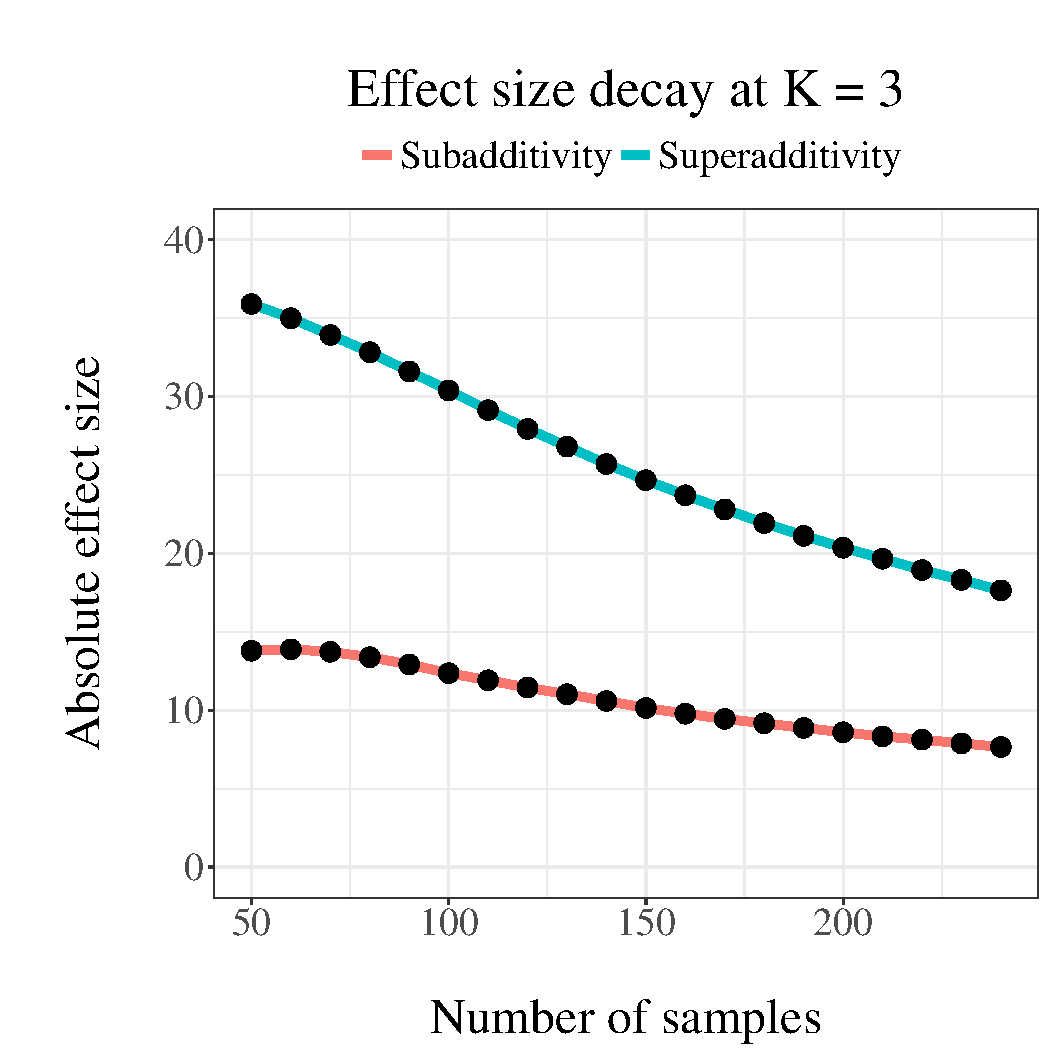
\includegraphics[scale = 0.5]{figures/compare3.pdf}
\caption{The effect size of subadditivity and superadditivity (calculated as the absolute difference between unpacked judgments and packed judgments, averaged over 200 chains) decays with increase in the number of samples taken. We plot this for $K = 3$ but this structure is maintained at all $K$. This plot shows that superadditivity decays faster than subadditivity with increase in the number of samples, and that subadditivity decays to close to zero with a smaller number of samples.}
\label{fig:decay}
\end{figure}
The size of the subadditivity and superadditivity effects decay with the number of hypothesis sampled. Subadditivity decays to almost zero with fewer samples than superadditivity as seen for the scene statistics model in Figure~\ref{fig:decay}. The time pressure in Experiment 1, by restricting the number of samples, may have rendered subadditivity observable, whereas the superadditivity effect is observable in both. Time pressure in Experiment 3 and cognitive load in Experiment 4 strengthened some of the effects, but did not consistently strengthen both effects. Thus, more experimental work is needed to understand the role of time pressure and cognitive load.
%end

Our results cannot be explained by simpler heuristics like anchoring and adjustment. Although anchoring to a low probability hypothesis can account for superadditivity (probability estimates are adjusted upwards), anchoring to a high probability example does not explain subadditivity, since the high probability hypothesis still has lower probability than the total probability of the focal space (e.g., the probability of ``chair'' is lower than the probability of seeing any object starting with the letter ``c''). Thus, adjustment away from the low probability hypothesis towards the normatively correct probability cannot lead to a probability estimate higher than the answer to the packed query (where presumably no anchoring occurs).

%start
Other effects like the conservatism bias could also potentially be captured by variants of our model. Conservatism bias has previously been modeled using noisy retrieval of memories \citep{Dougherty1999,marchiori15} and can be reproduced in our model in the same spirit by allowing noisy initialization. Due to the discreteness and resulting low resolution of probability estimates allowed by a limited number of samples, even a few initial samples from the focal space might over-represent its probability. When queried focal space has low probability, the chain is initialized there and the few initial hypothesis generated from the focal space could give it higher probability than the true posterior. When the queried focal space instead has high probability, it will be under-represented (as predicted by conservatism) if there are more samples from its complement space. If we introduce noise that causes the chain to initialize in the complement space with some small probability, this will produce a higher probability for the complement space and thus a lower  probability for the focal space---i.e., conservatism. That being said, the addition of noise might interfere with our explanations of other probability judgment biases, so further modeling work is needed to explore this hypothesis.
%end 

%Our experiment 2 however shows results that agree with \cite{super} on the effects that are observable for paradigms with "well defined categories" in showing that subadditivity is not observed, whereas superadditivity is. 

%To explain these effects, we focus on two properties, both of which are replicated in our model (a) Subadditivity is a weaker effect that superadditivity (see Figs \ref{fig:subadd}, \ref{fig:superadd} and \ref{fig:results1}), (b) these effects are time sensitive and reduce with increase in processing time (see Figs \ref{fig:subadd} and \ref{fig:superadd}), up until a resource rational threshold. The effects for our first experiment were expected to be of higher magnitude and in the 20 second time constraint, did not die out. Whereas in the second experiment,  due to constraints from the design of the experiments, the overall effects were expected to be of a smaller magnitude. Subadditivity is a weaker effect that superadditivity, and was washed out in the given time while superadditivity survived.
%While the effects in the experiments conducted by \cite{super} were designed to be as strong as possible (like our experiment 1), the participants were given no time constraints. We conjecture that the similarity between our results from experiment 2 and those from \cite{super} is obtained by the cancellation of two opposing effects (a) reduced typicality in our experiment that decreases the size of the effects, and (b) reduced processing time in our experiment that increases the size of the effects. Comparing our experiment 1 with \cite{super}, we see that only point (b) from before applies---i.e. the typicality is unchanged, but we include a constrain on processing time unlike \cite{super}---therefore the effect size of implicit subadditivity is increased in our experiment 1 and is observable.

\subsection{Optimal stopping}
\label{sec:MCMC_optimal_stop}

So far, we have assumed that the number of samples is constrained solely by the available time, but the computational rationality perspective argues that this number is chosen adaptively to balance the benefits of taking more samples against their costs in time and energy \citep{Gershman2015,Vul2014,griffiths2015}. Studying this experimentally would involve changing the incentive structure of the experiment in tandem with response deadlines and cognitive load manipulations.

To find the optimal stopping point, we need to compute the value of additional samples, and decide whether it outweighs the cost of taking these additional samples. A naive approach to finding with value of additional samples is to examine how much closer this gets us to the true posterior distribution. This however is circular, since the true posterior is what we are trying to approximate in the first place. We don't know it in advance in order to compare our current approximation with. We discuss this problem in Chapter \ref{chap:psych} in Section \ref{sec:psych_BR}, when considering concerns with current models of resource-rationality or computational rationality -- that knowing the optimal stopping point, in the most naive sense, can be more expensive that the original computation we set out to approximate. 

There are however ways to get around this for certain classes of rational-process models, including the sampling mechanism proposed here. To understand this, we first formalize the boundedly rational cost function. If the approximate posterior is given by

\begin{align}
P(h|d) \approx \hat{P}_N(h|d) = \frac{1}{N}\sum_{n=1}^N \mathbb{I}[h_n=h],
\end{align}

Then the bounded rationality objective function is a function of the distance $\mathcal{D}$ between this approximation and the true posterior, as well as the cost of the resources required to make this approximation, where we assume that cost scales linearly with the number of samples, with $\mathcal{C}$ per sample. This gives the following objective $\mathcal{F}$ that we wish to minimize as a function of the number of samples (N):
\begin{align}
\mathcal{F}(N) = \mathcal{D}[\hat{P}_N(h|d)||P(h|d)] + \mathcal{C}N
\end{align}
We choose the Kullback-Liebler (KL) divergence, or relative entropy, as the distance metric to get
\begin{align}
\mathcal{F}(N) &= \mathcal{D_{KL}}[\hat{P}_N(h|d)||P(h|d)] + \mathcal{C}N \\
& =  \sum_h \hat{P}_N(h|d) \log \frac{\hat{P}_N(h|d)}{P(h|d)} + \mathcal{C}N
\end{align}
Exactly computing this objective still requires the exact posterior to evaluate exactly. However, two insights make this a lot easier. First, we note that the KL divergence can we written as follows (see also Equation \ref{eq:ELBO}):
\begin{align}
\mathcal{D_{KL}}[\hat{P}_N(h|d)||P(h|d)]  = \sum_h \hat{P}_N(h|d) \log \frac{\hat{P}_N(h|d)}{P(h,d)} + \log P(d)
\label{eq:split_KL}
\end{align}
Here, the first term is computable since a) we know the joint distribution $P(h,d)$,  and b) we can take expectations over our approximate distribution $\hat{P}_N(h|d)$. The second term remains intractable. 

However, our second insight is that we don't need to compute the exact value of the objective function. Our objective function is a linear sum of smooth monotonic functions: the KL term decreases (on average) with increase in the number of samples, and the cost term increases. Therefore, our cost function is convex, and the global minimum can be found simply by following local gradients. This smooth, convex assumption does not hold for many other classes of resource-rational approximations, for example, if we are optimizing over the space of discrete strategies (eg. whether to employ a certain heuristic or another), rather than optimizing over an (almost) continuous parameter like the number of samples drawn. This local gradient (or the incremental value to one additional sample) is given by:
\begin{align}
\mathcal{F}(N + 1) - \mathcal{F}(N) =  \sum_h \hat{P}_{N+1}(h|d) \log \frac{\hat{P}_{N+1}(h|d)}{P(h|d)} -  \sum_h \hat{P}_N(h|d) \log \frac{\hat{P}_N(h|d)}{P(h|d)} + \mathcal{C}
\end{align}
Since the second term in Equation \ref{eq:split_KL} is the same in both, it cancels out, leaving a tractable expression for the gradient. The gradient can therefore be estimated locally everytime a new sample is drawn. Once this gradient starts to become negative, it is time to stop computations. This can be seen as treating the sample based approximation as a variational family and finding the optimal number of samples\cite{saeedi17}. See Chapter \ref{chap:approx}, Section \ref{sec:approx_var} for further details on variational approximations.

\subsection{Limitations and future extensions}

%Our model can be improved in several ways. particularly by better leveraging past experiences and run-time information. For example, improving the way the proposal distribution incorporates these. A proposal distribution is expected to be strongly affected by what has been learned from past experience i.e. from knowledge of the structure of the hypothesis space by which locality is determined, learning the prior and sometimes developing biases towards specific classes of hypotheses \citep{markantimpact}. A possible extension from this work is to think about other ways in which to organize the latent space rather than by brute force clustering (for example in \cite{kemp2009structured}), and how this organization is learned. Depending on the specific problem, the hypothesis space could be very differently organized, changing the locality metric, as well as by making various classes of hypotheses more or less accessible \citep{markantimpact}. Further, the proposal distribution does not incorporate any external information at run time. Which parts of the hypothesis space to focus on, as well as modulation of the step sizes of the proposal distribution in order to appropriately optimize exploration of the space, might depend on the specific case at hand and human behavior in these cases might be better modeled by incorporating the run-time data into the proposal distribution. Using data to drive the proposal distribution would result in weighting the likelihood higher than the prior, in resource-constrained runs\footnote{irrespective of initialization and proposal distribution, the Markov chain converges to the exact posterior asymptotically}. This might successfully model observed cognitive effects like base rate neglect.

Our model can be improved in several ways. First, we adopted relatively simple assumptions about initialization of the Markov chain. Recent work suggests that humans might use a fast, data-driven proposal distribution learned from previous experience \citep{Yildirim15,Gershman2014b}. We present a proposal mechanism of this sort in Chapter \ref{chap:LTI}.
%start2
This mechanism might capture effects that hinge on the availability and representativeness heuristics. Our current model fails to replicate these effects because it assumes that all hypotheses are equally likely to be proposed, although they are accepted proportional to their probability. A proposal distribution that preferentially proposes certain hypotheses might help build a link between our stochastic sampling-based method and the literature on heuristics.
%end2

%SG: I didn't get this part (how could our model predictions not depend on the typicality of the data??) so I took it out.
%Second, our simplistic assumptions about the proposal distribution could likewise be made more sophisticated by using data-driven methods. 
%start2
%Our model cannot replicate effects that hinge on the typicality of the observed data---the probability of the data does not influence the model predictions. However, some effects like the `enhancement effect' \citep{koehler1997enhancement} and explicit superadditivity \citep[where each unpacked hypotheses is evaluated with separate queries and then added together;][]{macchi1999note}, can be attributed to differences in the typicality of the observations on which the inference is being conditioned. These effects cannot be captured by our model in its current form. We expect that incorporating data-driven approaches to the proposal distribution might be able to induce this dependence on the typicality of the observed data.
%end2

%ES2: Below, we could also add something about why that also means that we can't just simply manipulate time in a continuously fashion in the experiments.

%This idea could potentially explain several cognitive biases not captured by our model, such as indirect priming effects \citep{mcnamara92} and the representativeness heuristic \citep{kahneman72}. As this initialization method incorporates the run-time data, it too might lead to weighting the likelihood more than the prior in resource constrained runs, giving base rate neglect.

%Another degree of freedom of our model is how strict or lenient the acceptance function is. One can modulate how likely the acceptance function is to accept states of lower probability by altering the `temperature' of the simulation \citep{hwang1988simulated} without losing the asymptotic exactness properties of MCMC Metropolis-Hastings. At high temperatures, the chain is more likely to accept lower probability hypotheses and vice versa for lower temperatures. How likely people are to explore the hypothesis space, and how likely they are to instead instead stay in one high probability mode, could reflect different values for this temperature parameter. This might help characterize differences in hypothesis search behavior between subjects or within subject depending on changing situations.

Our experiments and simulations only studied two domains (medical diagnosis and scene understanding), but there exist many real-world domains that impose a severe computational burden on mental inference. 
%start2
It is important again to point out here that we expect our model to work only in domains in which humans have natural intuitions for relative probabilities of hypotheses, without requiring explicit calculation. 
%end2
For example, it has been shown that humans are capable of simulating physical trajectories that they have never directly observed, making fairly accurate inferences when predicting the motion of a projectile \citep{motion}, judging mass in collisions \citep{collision}, and judging the balance of block towers \citep{blocks}. Furthermore, research also suggests that humans sample noisy simulations of future trajectories \citep{smith2013sources,hamrick2015think}, but the precise sampling mechanisms are currently unknown. The number of possible trajectories is exponentially large in this domain, and thus approximate inference schemes like MCMC may come into play.

% Needs a better written conclusion
%The scope of this work has been an attempt to further close the gap between optimal Bayesian models of cognition at the computational level and the biases and shortcomings we find when humans actually carry out inferences because of the algorithmic implementations of these computational ideas.

Returning to the puzzle we started with, why is it that humans are sometimes so successful at probabilistic inference, and at other times so unsuccessful? We have identified one common source of inferential fallacies: computational constraints on hypothesis generation. Although this account can explain many departures from rationality, it remains puzzling why humans should fail at tasks where the hypothesis space is clearly and exhaustively enumerated---for example, in tasks that involve inferences about balls in urns \citep[see][for a review]{peterson1967man}. We suspect that people have difficulty with these tasks because their artificiality invokes an explicit, error-prone reasoning process (much like solving a math problem) rather than drawing upon intuitive knowledge of natural domains \citep{evans02,cohen16}. Studies have shown that difficult inference problems can be transformed into tractable ones simply by providing subjects with an intuitive causal structure \citep{tversky80,krynski07,cheng85}. A direct comparison between naturalistic and artificial versions of the tasks we used in our studies is challenging because scene knowledge is complex and high-dimensional (precisely why we were interested in this domain to begin with). Thus, our claims remain tentative until further experimentation yields decisive evidence.